\documentclass[a4paper,11pt]{report}
\usepackage{ucythesis}
%\usepackage{latexsym}
\usepackage{times}
\usepackage{amsmath}
\usepackage{graphicx}
\usepackage{float}
\usepackage{subfig}
\usepackage{algorithm}
\usepackage{algpseudocode}

\begin{document}
%\phddissertation %\msthesis for master degree
\msthesis

\title{DIGITAL MATTING AND COMPOSITING}
\author{Savvas Christodoulou}
%\fulldegs{}
%\fulldegs{M.S. major, university, year\\\vspace{0.5em}
%B.S., major, university, year}
%\degs{B.Sc.}
%\degs{M.S., B.S.}
\monthcom{June} %\month of completion
\majoradviser{Yiorgos Chrysanthou}
\associateadviser{Constantinos Pattichis}
\associateadviser{Paris Kaimakis}
%\associateadviser{Committee Member's Name}
%\associateadviser{Committee Member's Name}
\copyrightyear{2014} %\basically the completion year

\begin{abstract}
Digital image matting refers to the area of computer vision that attempts to solve the problem of separating the foreground from the background and compositing it to and new background. Traditional image segmentation algorithms make a hard segmentation of multiple regions in an image, whereas in alpha matting fuzzy regions are taken into account as mixed regions and fractional values are estimated to form an alpha matte that is used for compositing. The standard method for matting used in the industry is blue screen matting, where the background is monochrome, usually green or blue. Recent research focuses on solving the problem of natural image matting, where the background consists of a variety of colours. Natural image matting is an ill-posed problem, where for a given image we have multiple solutions. The under constrained nature of the problem requires prior input, usually a user provided trimap or a set of scribbles. 
Bayesian matting was a first attempt to solve the matting problem, which uses a Bayesian framework, and another basic approach is Closed Form matting where the Colour Line Model is assumed to estimate alpha and the notation of a Matting Laplacian Matrix is introduced. Other methods include consideration of pixel affinities and image gradient, use of depth or texture information as priors, use of more sophisticated sampling methods, and the use of better classification algorithms. Matting has been extended to video, where trimaps are automatically generated and temporal coherence of alpha values is considered. Other research approaches consider the use of custom hardware to solve the matting problem. 
In this thesis I present the work done to develop a matting system that consists of a new matting algorithm and the extension of it to an application with the use of Microsoft’s Kinect sensor. Execution times are promising for a real time application using GPU hardware. Future work consists of the use of the new Kinect 2 sensor and consideration of illumination sources in natural images to improve the matting and compositing method. 
\newline
\centerline{Savvas Christodoulou -- University of Cyprus, 2014}

\end{abstract}

\beforepreface %\required

\acknowledgement 
I would first like to thank my fellow student Mr. George Georgakis that was involved in the early stages of the project that this thesis is based upon. His excellent knowledge in the areas of computer vision and image processing along with his exceptional analytical and programming skills were very helpful in development of many of the ideas during the experimental process. 
I would also like to thank lab assistant Mr. Ioannis Konstantinou, an expert in the areas of image/video processing and computer vision, that offered guidance and recommended many ideas. 
Last and most importantly I would like to thank my supervisor Dr. Yiorgos Chrysanthou for the initial motivation and conceptualization the whole project and his consultation during various phases of the research process.

%\credits %\ Publications that lead to this thesis (if any)

\afterpreface %\required

%chapers and sections%%%%%%%%%

\chapter{Introduction}
\label{chap:intro}

\section{Motivation}
\label{sec:motivation}

In recent years the area of Computer vision, also known as Machine vision has attracted interest both in academia and in commerce. Most major universities are offering computer vision courses and research degrees and conferences and journals are accepting more computer vision related papers. Computer vision combines a variety of subjects such as Artificial intelligence, Machine Learning, Image, Video and general Signal Processing and other areas from computer science and engineering. Recently we have seen more commercial uses of computer vision technology, such as augmented reality applications in home computers, mobile devices, and in home entertainment. In its early stages, computer vision was mainly used for robotics in an attempt to make an artificially intelligent machine that can “see” not only passively but actually understand the content of the information it gathers. In subsequent years computer vision research had been extended for uses in medical image processing, photography and cinema. The emergence of computer graphics in films along with the appearance of the personal computer that allowed the users to manipulate computer graphics and digital images, opened the path for new digital image processing methods to be developed and the area of computer vision got more involved in this process, since computer vision for robotics could not actually be applied in the industry yet. 
\par
Segmentation has always been a difficult problem in computer vision and numerous approaches to solve this problem have been developed and can be found in the literature. In the industry, specifically in cinema, segmentation of portions of a film frame plays crucial role for the creation of synthetic scenes. In the early analog years, film producers had to manually cut and composite objects on film frames to create synthetic scenes and later on in the digital age, methods were pioneered to digitally segment and composite objects in scenes \cite{compositing}. Computer vision is still a developing area and since it is already applied for commercial purposes, any contribution to it is welcome.

\section{History}
\label{sec:history}

As mentioned before, in the early digital years, the film industry started to seek ways to create visual effects and wanted to combine captured film frames with synthetic objects, scenes generated with computer graphics, or combine pre-existing scenes with others. \textit{Lucasfilm}, creators of the Star Wars movies were ahead of their time in terms of visual effects and made important contributions to the film industry. Specifically in 1984 \cite{compositing} they introduced a method for compositing four channel images using a matte component, or better known as \textit{alpha matte}. During the same period, computer graphics research had reached a point that computer generated imagery could effectively be used in movies. In 1996 \textit{Microsoft Research} introduced a method for separating foreground from background objects efficiently using a monochrome background \cite{blue}, also known as \textit{chroma key}. In most of the cases blue or green colours are used for the background, due to the fact that they are the furthest from human skin colour and also take advantage of \textit{bayer grid} properties. They also introduced the \textit{triangulation} method where the same foreground was photographed with different natural backgrounds in order to create the alpha matte \cite{blue}. Another contribution took place in 1999 \cite{environment} where transparent and translucent objects refractive properties were taken into account for the distortion of the background during compositing. From there on digital matting and compositing have been the most important factor for visual effects in movies. The emergence of image and video editing software took advantage of the same techniques, and digital image matting and compositing started to make its appearance in other areas such as photography. Recent matting research focuses on solving the problem of matting on natural images, where background colours are unknown. 

\section{Terminology}
\label{sec:terminology}

Matting is the process where given an image \textit{C}, the goal is to separate the foreground \textit{F} from the background \textit{B} and create an alpha matte $\alpha$. The alpha matte is usually a single channel image where \textit{0} values are considered background, \textit{1}’s are considered foreground and intermediate values are considered to be the blending factor for the fuzzy regions/mixed pixels in the image. Compositing is the process of using the estimated alpha matte to composite the foreground and fuzzy parts of the image to a new background. In this case the alpha matte plays the role of the fourth channel of the foreground image called alpha channel. The whole idea is formulated using equation (\ref{eq:composite_e}). 

\begin{equation} \label{eq:composite_e}
C=\alpha F+(1-\alpha)B
\end{equation}

Assuming that an image consists of three channels, red \textit{R}, green \textit{G} and blue \textit{B} and an alpha channel $\alpha$, the problem is severely under constrained with three equations and seven unknowns (\ref{eq:composite_ce}) and no single solution can be found. 

\begin{equation} \label{eq:composite_ce}
C_r=\alpha F_r+(1-\alpha)B_r,\;\; C_b=\alpha F_b+(1-\alpha)B_b,\;\; C_g=\alpha F_g+(1-\alpha)B_g
\end{equation}

Such a problem could be solved only with some prior information and so, in most natural image matting methods the concept of a trimap (Figure 1b) is introduced that can be either user provided, or generated automatically. The trimap is a single channel image that consist of three regions, definite foreground, definite background and unknown region. The unknown region usually consists of the edges of the object to be segmented in the image and the fuzzy regions such as hair, fur, motion blur etc.

\begin{figure}[t!]
\centering
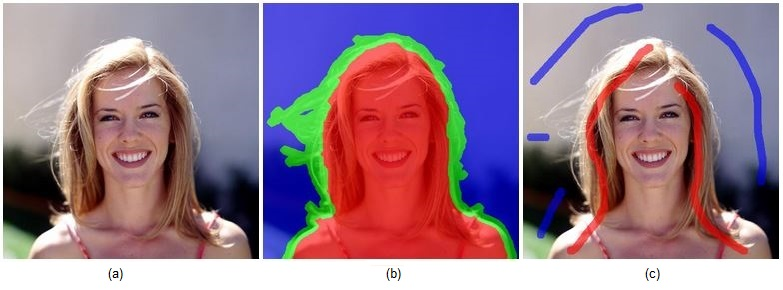
\includegraphics[width=0.9\columnwidth]{Chapter1/1/trimap.jpg}
\caption[Natural image, trimap and scribbles.]{A natural image, the trimap with definite foreground in red, definite background in blue and unknown region in green and an illustration of scribbles.}
\label{fig:trimap}
\end{figure}

\section{Overview of thesis}
\label{sec:overview-of-thesis}

The rest of the thesis is organized as follows: the following chapter is a literature review of various image matting methods, including fundamental methods such as blue screen matting, an in depth explanation of natural image matting methods starting from basic ones such as Bayesian matting and Closed Form matting and then a description of other important matting methods. The next section discusses state of the art matting methods, followed by a review of video matting techniques. The last section of the literature review consists of analysing matting methods with custom or specialized hardware. The next chapter gives a brief description of the development tools used for experimental implementation purposes. Chapter 4 describes all the preliminary work; the initial pre-existing algorithms used and early segmentation and matting algorithm formulations. A detailed description of the final algorithm and results from tests on benchmark images along with visual performance comparisons with other algorithms is done in Chapter 5. Chapter 6 presents an application of our algorithm using the Microsoft Kinect sensor, and a description of the extensions made to the algorithm for automatic trimap generation. Results are presented using images taken from the sensor, and visual performance comparisons are done with other algorithms. The final chapter consists of future work and conclusions.
\chapter{Natural Image Matting }
\label{chap:natural-image-matting}

\section{Introduction to matting}
\label{sec:introduction-to-matting}

A basic formulation that compositing is based on \cite{compositing} can be defined as follows: given the foreground colour \textit{F=\(F_r,F_b,F_g\)}, the background colour \textit{B=\(B_r,B_b,B_g\)} and $\alpha$, for each pixel the compositing operation is defined by \textit{C=$\alpha$F+(1-$\alpha$)B}. The \textit{RGBA} quadruple for the foreground pixels to be composited, with first three values the colour channels and the fourth value the alpha channel, can be represented for example as \textit{(1,0,0,1)} for an opaque red pixel, \textit{(0,0,1,0.5)} for a blue semi-transparent pixel or \textit{(0,1,0,0)} for a green transparent pixel. So, taking as an example the second case the compositing equation (\ref{eq:composite_e_e}) could be solved as:

\begin{equation} \label{eq:composite_e_e}
\begin{split}
F=(0,0,0),\;B=(0,0,1),\;\alpha=0.5,\;C=?,\\
C_r=0,\;C_g=0,\;C_b=0.5 \times 0+(1-0.5) \times 1\;
\Rightarrow\;C_g=0.5,\\
C=(0,0,0.5)
\end{split}
\end{equation}

So by compositing a black foreground pixel with a blue background pixel and by using a semi–transparent alpha value for the foreground, the resulting pixel in the composite is basically a dark blue pixel.
\par
Matting is the inverse problem; assume that you have an image that is composited with foreground \textit{F} and background \textit{B}. Given an image colour \textit{C}, find \textit{F}, \textit{B} and \textit{$\alpha$} so \textit{C=$\alpha$F+(1-$\alpha$)B} is valid. Since \textit{F} or \textit{B} distinct values aren’t prior known, the equation has multiple solutions. In \textit{Blue Screen Matting} \cite{blue} the image is given and the background colour is known (\textit{chroma key}). So assuming that the foreground does not have chroma key colours within it, eliminating chroma key values from the equations i.e. setting them to zero, will produce the foreground. This is the most extensively used method in films, since the background of a scene can be easily set to a single colour (Figure 2).

\begin{figure}[t!]
%\centering
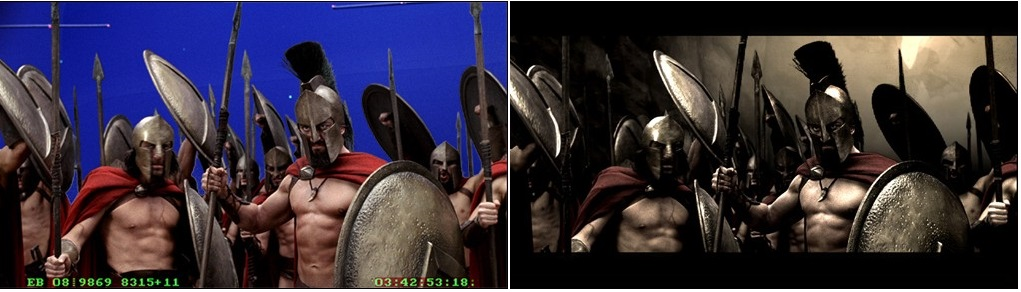
\includegraphics[width=1\columnwidth]{Chapter2/2/bluescreen.jpg}
\caption[Blue screen used in the movie 300.]{Blue screen used in the movie 300. The film was shot using the digital backlot technique, where the whole movie shooting took place in front of blue backgrounds.}
\label{fig:bluescreen}
\end{figure}

Another approach is having two images with the same foreground but different backgrounds, assuming that the two images are completely aligned. In this case the \textit{triangulation} method is used by creating a matrix with six equations and four unknowns and the solution of it gives the \textit{RGB} and $\alpha$ values for the foreground pixels \cite{blue}. The triangulation method is typically used for still images since it would not be practical for film purposes. 
In natural image matting we have an image \textit{I} or composite \textit{C} but no knowledge of foreground \textit{F} and background \textit{B} components. As mentioned in the previous chapter this is an under constrained problem and prior information must be used. 

%%%%%%%%%%%%%%%%%%%%%%%%%%%%%%%%%%%%%%%%%%%%%%%%%%%%%%%%%%%%%%%%%%%%%%%%
\section{Bayesian matting}
\label{sec:bayesian-matting}

In 2001 a research team including well-known computer vision researcher Szeliski, attempted to solve the natural image matting problem using a Bayesian framework \cite{bayesian}. The idea is that given an image \textit{C}, for each pixel find the foreground, background and alpha values that maximize the probability of observing the pixel’s colour (\ref{eq:bayesian_e_a}). Using Bayes rule (\ref{eq:bayesian_e_b}), we have the following formulation:

\begin{subequations}\label{eq:bayesian_e}
\begin{equation}\label{eq:bayesian_e_a}
arg\;\underset{F,B,a}{max}\;P(F,B,\alpha\mid C)
\end{equation}
\begin{equation}\label{eq:bayesian_e_b}
= arg\;\underset{F,B,a}{max}\;P(C\mid F,B,\alpha)P(F)P(B)P(\alpha)/P(C)
\end{equation}
\begin{equation}\label{eq:bayesian_e_c}
= arg\;\underset{F,B,a}{max}\;L(C\mid F,B,\alpha)+L(F)+L(B)+L(\alpha)
\end{equation}
\end{subequations}

Notice that the probability of the image is disregarded since it is constant and doesn’t affect any of the other terms (\ref{eq:bayesian_e_c}). Also F, B and $\alpha$ terms are treated independently and the problem is then expressed as a sum of log probabilities (\ref{eq:bayesian_e_c}). The first term is considered the data term and is modelled with (\ref{eq:bayesian_e_2}), and the other terms are the prior probabilities and are modelled via (\ref{eq:bayesian_e_3}).

\begin{equation} \label{eq:bayesian_e_2}
L(C\mid F,B,\alpha)=-\left \| C-\alpha F-(1-\alpha)B \right \|^{2}/\sigma_{C}^{2}
\end{equation}

\begin{equation} \label{eq:bayesian_e_3}
L(F)=-(F-\overline{F})^{T}\Sigma _{F}^{-1}(F-\overline{F})/2
\end{equation}

In (\ref{eq:bayesian_e_2}) sigma is a tunable parameter and in (\ref{eq:bayesian_e_3}) the covariance matrix and mean can be computed by samples collected based on the trimap. \textit{F} is substituted by \textit{B} to get the log likelihoods of background and $\alpha$ likelihood is initially considered to be constant. Figure 3 is a visualization of the idea.

\begin{figure}[t!]
%\centering
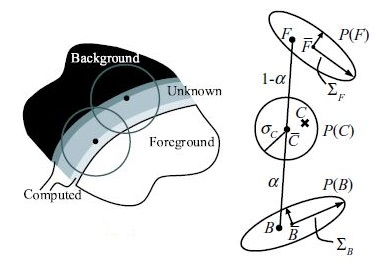
\includegraphics[width=0.5\columnwidth]{Chapter2/2/bayesian_figure_1.jpg}
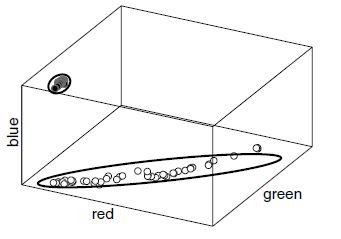
\includegraphics[width=0.5\columnwidth]{Chapter2/2/bayesian_figure_2.jpg}
\caption[Foreground and background distributions.]{Trimap (left) with corresponding distributions (middle). Distributions of foreground and background colours in RBG colour space are fitted within ellipses (right). Figures taken from \cite{bayesian} and \cite{visualeffects}.}
\label{fig:bayesian_e_f_4}
\end{figure}

By substituting the equations (\ref{eq:bayesian_e_2}) and (\ref{eq:bayesian_e_3}) and solving them by taking partial derivatives,\textit{ F} and \textit{B} are estimated assuming that $\alpha$ is constant. On the other hand, assuming that \textit{F} and \textit{B} are constant, (\ref{eq:bayesian_e_4}) is used to estimate $\alpha$. The two methods are alternated until estimated \textit{F}, \textit{B} and $\alpha$ converge.

\begin{equation} \label{eq:bayesian_e_4}
\alpha =\frac{(\textbf{C}-\textbf{B})\cdot (\textbf{F}-\textbf{B}))}{\left \| \textbf{F}-\textbf{B} \right \|^{2}}
\end{equation}

The problem that arises from this formulation is that modelling colour distributions in natural images cannot be done with a simple probability density function, because in natural images the distributions will possibly be overlapping. A proposed solution is to model the distributions as a mixture of Gaussian distributions (Figure 4).

\begin{figure}[t!]
\centering
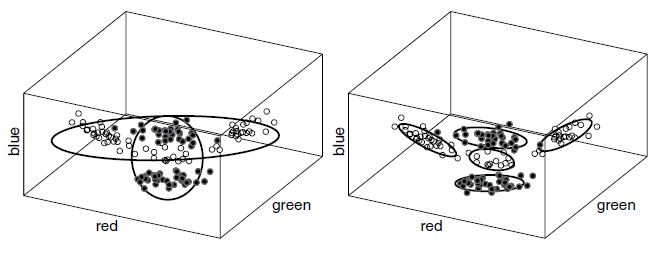
\includegraphics[width=0.8\columnwidth]{Chapter2/2/bayesian_figure_3.jpg}
\caption[Overlapping distributions.]{Overlapping F and B colour distributions (left). F and B colour distributions fitted into multiple ellipses (right). Figure taken from \cite{visualeffects}.}
\label{fig:bayesian_figure_3}
\end{figure}

%%%%%%%%%%%%%%%%%%%%%%%%%%%%%%%%%%%%%%%%%%%%%%%%%%%%%%%%%%%%%%%%%%%%%%%%%%%%%%%%%%%%%%%%%%%%
\section{Closed Form matting}
\label{sec:closed-form-matting}

Another major contribution to solving the matting problem was introduced in 2008 by Levin et al \cite{closedform} where an observation made in natural images lead to the assumption that within a small window around a pixel, pixel values in \textit{RGB} colour space lie on straight lines. This idea is called the \textit{colour line model} and can be visually represented in Figure 5a. If \textit{$C_{i}$} is a colour pixel and \textit{$B_{0}$} is a background pixel within a colour line, $\alpha_{i}$ can be estimated by (\ref{eq:closed-form-e1}). $\alpha_{k}$ is the vector connecting the foreground and background colour lines (Figure 5c).

\begin{equation}\label{eq:closed-form-e1}
\alpha_{i}=\textbf{$\alpha_{k}$}\cdot (\textbf C_{i}-\textbf B_{0})= \alpha _{k} \cdot \textbf{C}+b_{k}
\end{equation}

\begin{figure}[t!]
\centering
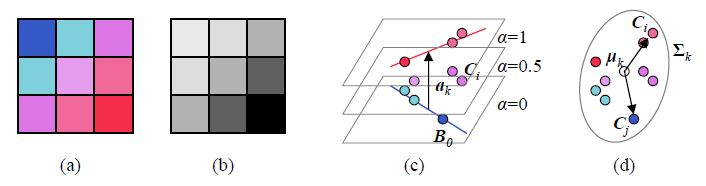
\includegraphics[width=1\columnwidth]{Chapter2/2/closed_form_figure_1.jpg}
\caption[Colour line model and alpha superposition.]{Colour line model and alpha superposition. A 3x3 window in an image with colour values (a) and intensity values (b). The pixels fitted to colour lines in RBG space and the superposition of a (c). Figure taken from \cite{algorithmsapplications}.}
\label{fig:closed-form-f1}
\end{figure}

A cost minimization function for all estimated a values over all windows is formulated in (\ref{eq:closed-form-e2}) where $\epsilon$ is a regularization term for overlapping distributions. For each window the energy function is simplified leading to (\ref{eq:closed-form-e3}), where \textit{L} is the \textit{Laplacian matrix} or \textit{matting Laplacian} and can be determined by (\ref{eq:closed-form-e4}); $\delta_{i,j}$ is the Kronecker delta, \textit{M} is the number of pixels in each (overlapping) window, \textit{$\mu_{k}$} is the mean colour of the pixels in window \textit{$W_{k}$}, and \textit{$\Sigma_{k}$} is the 3x3 covariance of the pixel colours (Figure 5d).

\begin{equation} \label{eq:closed-form-e2}
E_{\alpha}=\sum_{k}(\sum_{i\in W_{k}}(\alpha_{i}-\alpha_{k}\cdot C_{i}-b_{k})^2)+\epsilon\left \| \alpha_{k} \right \|)
\end{equation}

\begin{equation} \label{eq:closed-form-e3}
E_{\alpha}=\alpha^T\textbf{L}\alpha
\end{equation}

\begin{equation} \label{eq:closed-form-e4}
L_{ij}=\sum _{k:(i,j)\in W_{k}}(\delta _{ij}-\frac{1}{M}(1+(C_{i}-\mu _{k})^T\hat\Sigma_k ^{-1}(C_{j}-\mu _{k})))
\end{equation}

The user provided scribbles for definite foreground and definite background pixels, provide the energy function some prior a values, so only a sparse set of linear equations has to be solved. When $\alpha$’s are calculated, the foreground and background colours are estimated using a least squares minimization of the compositing equation regularized with a spatially varying first order smoothness (\ref{eq:closed-form-e5}). $\lambda\left |\bigtriangledown \alpha_{i}  \right |$ weights separately the x and y components of the F and B derivatives.


\begin{equation} \label{eq:closed-form-e5}
E_{B,F}=\sum _{i}\left \| C_{i}-[\alpha+F_{i}+(1-a_{i})B_{i}] \right \|^{2}+\lambda\left |\bigtriangledown \alpha_{i}  \right |(\left \| \bigtriangledown F_i \right \|^{2}+\left \| \bigtriangledown B_{i} \right \|^2)
\end{equation}

Another observation made by the authors, was that even before user information about the image was provided, the \textit{eigenvectors} of the matting Laplacian corresponding to the smallest \textit{eigenvalues}, reveal a surprising amount of information about potentially good mattes. They subsequently proposed an algorithm called \textit{Spectral matting} \cite{spectral} were the \textit{K} smallest eigenvectors are used as matting components to form a full matte (Figure 6).

\begin{figure}[t!]
\centering
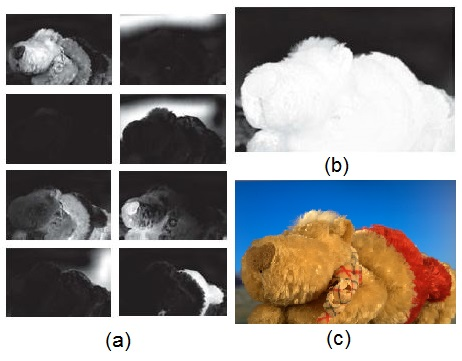
\includegraphics[width=0.8\columnwidth]{Chapter2/2/closed_form_figure_2.jpg}
\caption[Eigenvector images.]{In Spectral matting the eigenvectors that correspond to the smallest eigenvalues (a) can be used as matte components. The combination of them leads to a full matte (b) when compared to the image (c). Figure taken from \cite{spectral}.}
\label{fig:closed-form-f2}
\end{figure}

%%%%%%%%%%%%%%%%%%%%%%%%%%%%%%%%%%%%%%%%%%%%%%%%%%%%%%%%%%%%%%%%%%%%%%%%%%%%%%%%%%%%%%%%%%5
\section{Other matting methods}
\label{sec:other-matting-methods}

Although Bayesian and Closed Form matting had shown promising results, they were still struggling for highly transparent images or images with similar foreground and background colours. The fact that they were well formulated though, gave path for other methods to be developed. Besides using a probabilistic framework or a matting Laplacian, researchers took methods used in other computer vision areas and tailored them for the matting problem. 
An interesting approach is the use of the \textit{gradient} of the image in a method called \textit{Poisson matting} \cite{poisson}. First the spatial gradient of the matting equation is taken (\ref{eq:poisson-1}), typically in the intensity channel of the image, and if the foreground and background are relatively smooth compared to $\alpha$ i.e. $\alpha\bigtriangledown F+(1-\alpha)\bigtriangledown B$ is close to 0, the matte gradient will be proportional to the image gradient and the matte gradient can be approximated by (\ref{eq:poisson-2}). 

\begin{equation} \label{eq:poisson-1}
\bigtriangledown I=(F-B)\bigtriangledown \alpha+\alpha\bigtriangledown F+(1-\alpha)\bigtriangledown B
\end{equation}

\begin{equation} \label{eq:poisson-2}
\bigtriangledown \alpha\approx \frac{1}{F-B}\bigtriangledown I
\end{equation}

This formulation gives a differential equation for $\alpha$ in the unknown region and the minimization of it using information from the trimap, is the same as solving a \textit{Poisson equation} with the same boundary conditions. This method works well with images where background and foreground are both smooth but fails when an image foreground or background has strong gradients.
\par
Wang and Cohen \cite{iterativeoptimization} observed the issue with highly transparent images and the problems caused by a trimap with large unknown regions, so they proposed a \textit{belief propagation} method to determine alpha values. Pixels are marked and grouped. The initial marked pixels are the ones provided by the user as scribbles. Gaussian mixture models are computed for foreground and background pixels that are marked. Then for all pixels that are unmarked: a spatial distance transform is applied to a number of marked pixels and the closest unmarked pixels are marked. A \textit{Marcov Random field} is built based on marked pixels and for each node within it, samples from foreground and background colours are taken and the data cost is computed. Then the belief propagation algorithm is used to estimate a matte for the pixels in the graph and the uncertainty and the estimated foreground and background colours for each pixels in the graph are updated. The marked pixels group is also updated. Experimental results showed a better performance in highly transparent images when using scribbles combined with this method rather than a trimap (Figure 7).

\begin{figure}[t!]
\centering
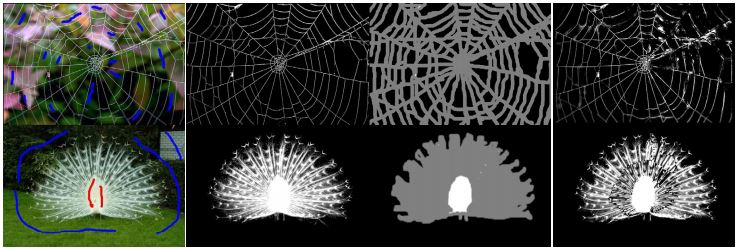
\includegraphics[width=1\columnwidth]{Chapter2/2/2_4_figure_1.jpg}
\caption[Iterative optimization matting results.]{Image alpha mattes are calculated using scribbles and trimaps using the \textit{Iterative Optimization} matting method. Using belief propagation, scribbles produce a better results for images with high transparency. Figure taken from \cite{iterativeoptimization}.}
\label{fig:iterative-optimization-f}
\end{figure}

The same authors a few years later proposed another method \cite{robust} that analysed the confidence of sampled pixels. Assuming that a trimap is provided, for each pixel in the unknown region a number of samples from foreground and background is taken as candidates for estimating foreground and background colours. From the candidates, good samples are considered the ones that as pairs of foreground and background pixels explain the mixed foreground background pixels as linear combinations. A \textit{distance ratio R} is defined (\ref{eq:robust-1}) between sampled pairs and the pixel that is examined, where lower is better. 

\begin{equation} \label{eq:robust-1}
R_{d}(F,B)=\frac{\left \| C-(\alpha F+(1-\alpha)B) \right \|}{\left \| F-B \right \|}
\end{equation}

Another consideration in this method, is the spread of sampling along the boundaries of the unknown region (Figure 8) instead of the spatially close, so colour variation can be taken into account.

\begin{figure}[t!]
\centering
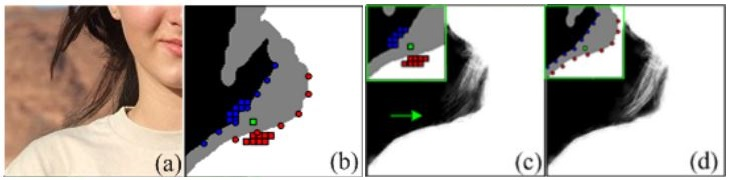
\includegraphics[width=1\columnwidth]{Chapter2/2/robust_figure_1.jpg}
\caption[Robust matting sampling strategy.]{\textit{Optimized colour sampling for robust matting} sampling strategy. Samples are gathered sparsely from the unknown region boundary and densely close to the unknown region. Figure taken from \cite{robust}.}
\label{fig:robust-f1}
\end{figure}

They also proceed to refine the estimated matte by assuming local smoothness, assuming that estimated $\alpha$’s with high confidence are correct and using them in a graph based labelling model.
The algorithm was further refined to a method called \textit{Soft Scissors} \cite{softscissors} that incrementally solved the matte based on user input. The matte is basically solved in real time; the user can brush along a foreground object’s boundary and the resulting alpha values can be viewed. An interesting fact is that the brush size that the user hovers over the image grows depending on the size of the mixed pixel region as seen in Figure \ref{fig:robust-f3}. An overview of the method can be seen in Figure \ref{fig:robust-f2}. 

\begin{figure}[t!]
\centering
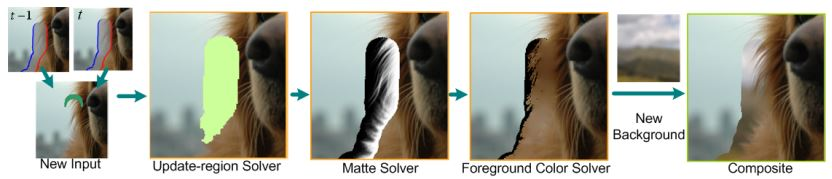
\includegraphics[width=1\columnwidth]{Chapter2/2/robust_figure_2.jpg}
\caption[A flow chart of Soft Scissors workflow.]{A flow chart of \textit{Soft Scissors} workflow. Figure taken from \cite{softscissors}.}
\label{fig:robust-f2}
\end{figure}

\begin{figure}[t!]
\centering
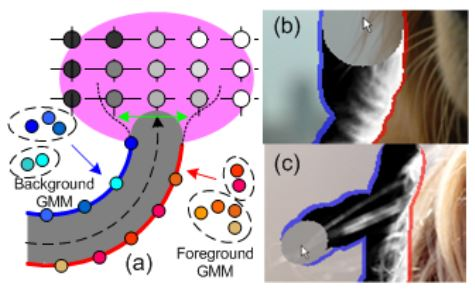
\includegraphics[width=0.7\columnwidth]{Chapter2/2/robust_figure_3.jpg}
\caption[Soft scissors automatic brush width adjustment.]{\textit{Soft scissors} automatic brush width adjustment. Figure taken from \cite{softscissors}.}
\label{fig:robust-f3}
\end{figure}

Another observation made by Gastal and Oliviera \cite{shared}, was that nearby pixels share similar foreground, background and $\alpha$ values and thus extra computation can be avoided, leading to a real time approach. The first step is basically to expand the trimaps’ known regions based on pixel affinities. For the sampling process, spatially close sample pairs are taken as illustrated in Figure 11. Then, the matte is estimated and locally smoothed using a smoothness algorithm.

\begin{figure}[t!]
\centering
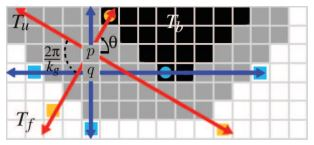
\includegraphics[width=0.6\columnwidth]{Chapter2/2/shared_figure_1.jpg}
\caption[\textit{Shared sampling for real-time alpha matting} sampling strategy.]{In \textit{Shared sampling for real-time alpha matting}, the spatially closest samples are selected. Each unknown pixels sample via different paths. Figure taken from \cite{shared}.}
\label{fig:shared-1}
\end{figure}

%%%%%%%%%%%%%%%%%%%%%%%%%%%%%%%%%%%%%%%%%%%%%%%%%%%%%%%%%%%%%%%%%%%%%%%%
\section{Latest matting methods}
\label{sec:latest-matting-methods}

After multiple methods were proposed to solve the matting problem, algorithms were still struggling to give satisfying results. The problem is that natural images are so variable that it is difficult to formulate a solution that works for every case. So far researches used their own datasets and there were no actual comparisons between methods. So the need for a standardized benchmark dataset led to the creation of a perceptual benchmark website \cite{benchmark} that offered datasets for researchers to use and performance evaluations both metric and visual. The error measures used are \textit{sum of absolute differences} SAD, \textit{mean square error} MSE, a \textit{gradient} measure and a \textit{connectivity} measure. The datasets consist of eight test images that are used for the performance comparisons, and twenty six train images with their respective ground truths that are used for training purposes. All images are provided in high and low resolutions, with variable amounts of transparency in each image and different types of trimaps; with wide unknown regions and with narrow. Since the matting problem was already well formulated but with unsatisfying results, from there on research focused on improving the quality of estimated mattes rather than on new mathematical formulations. In this section some of the state of the art methods for natural image matting are presented.
\par
Most matting algorithms assume pixel affinities either for sampling, for selecting the best foreground and background tuple, or for the alpha matte refinement. In \cite{nonlocal} the authors use the \textit{non-local} principle in an attempt to reduce user effort and provide an improved matting method over other ones that use scribbles instead of a trimap. This method is based on the \textit{non-local means} algorithm that is used for image denoising, in combination with the matting principles from \cite{closedform}. The idea is that instead of using pixels that are neighbouring to a pixel, use a weighted average of pixels that are considered to be the most similar. Figure 12 demonstrates the trimap generation by creating graph clusters and by using sparse user input.

\begin{figure}[t!]
\centering
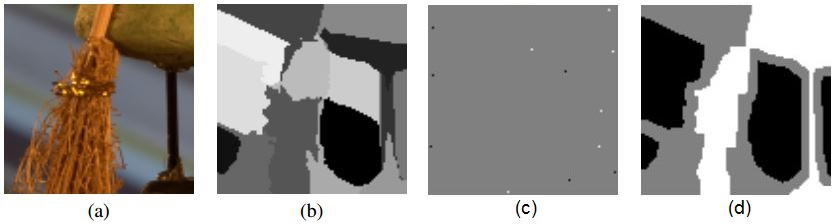
\includegraphics[width=1\columnwidth]{Chapter2/2/nonlocal_figure_1.jpg}
\caption[Non-local matting trimap generation.]{\textit{Non-local matting} trimap generation. Input image (a). Clusters (b). Sparse user input (c). Resulting trimap (d). Figure taken from \cite{nonlocal}.}
\label{fig:nonlocal-1}
\end{figure}

In \textit{KNN matting} \cite{knn} the authors use the idea of non-local matting, but instead of using the colour line model assumption from \cite{closedform}, they use a \textit{k-nearest neighbour} approach and also extract multiple alpha mattes as image layers. Their method uses a \textit{feature vector} (\ref{eq:knn-e1}) to represent pixels and depending on the scenario, different colour spaces are used along with pixel spatial information. In their article, they mention the usage of the HSV colour space with Hue \textit{h}, Saturation \textit{s} and Value \textit{v}. For each pixel in the unknown region the \textit{k-nearest neighbours} are selected (Figure 13) in the feature space using a kernel function defined in (\ref{eq:knn-e2}) and depending on the values of k, the layers of foreground and background can be extracted (Figure 14) and graph clusters can be created for each pixel.

\begin{equation} \label{eq:knn-e1}
X(i)=(cos(h),sin(h),s,v,x,y)_{i}
\end{equation}

\begin{equation} \label{eq:knn-e2}
K(i,j)=1-\frac{\left \| X(i)-X(j) \right \|}{C}
\end{equation}

\begin{figure}[t!]
\centering
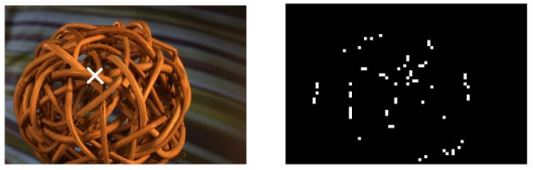
\includegraphics[width=1\columnwidth]{Chapter2/2/knn_figure_1.jpg}
\caption[KNN sampling strategy.]{\textit{KNN matting} sampling strategy. For a selected pixel (left) KNN collects samples (right) using a non-local method. Figure taken from \cite{knn}.}
\label{fig:knn-f1}
\end{figure}

\begin{figure}[t!]
\centering
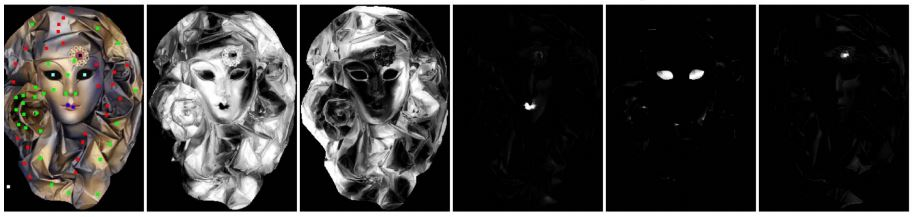
\includegraphics[width=1\columnwidth]{Chapter2/2/knn_figure_2.jpg}
\caption[KNN input clicks for alpha-mask extraction]{\textit{KNN matting} input clicks for alpha-mask extraction. Different input clicks are needed for different mask extraction. Figure taken from \cite{knn}.}
\label{fig:knn-f2}
\end{figure}

\begin{figure}[t!]
\centering
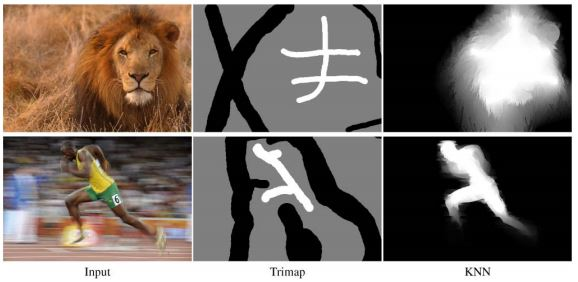
\includegraphics[width=1\columnwidth]{Chapter2/2/knn_figure_3.jpg}
\caption[KNN performance on fuzzy regions.]{\textit{KNN matting} performs poorly on images with a high amount of mixed pixels. Figure taken from \cite{knn}.}
\label{fig:knn-f3}
\end{figure}

A common problem that occurs in natural image matting, is estimating $\alpha$ in the case where foreground and background colour distributions are overlapping. In this case foreground and background regions cannot be distinguished and sampling methods using common colour spaces fail. A method proposed \cite{texture} to tackle this issue was the combination of colour features with \textit{texture features}. The texture feature is a combination of \textit{chromatic} and \textit{structural} content of the image. For the chromatic texture features, the image is smoothed using \textit{bilateral filters} that preserve image edges, and obtain a high, medium and low smoothing of the image. The structural texture feature is obtained through \textit{Haar wavelet decomposition} of the image into four sub images. The feature vector is formulated as:

\begin{equation} \label{eq:texture-e1}
FV_{T}=\{A^{grad}_{(l,c)}, A^{var}_{(l,c)}, A^{mean}_{(l,c)}, H^{mean}_{(l,c)}, V^{mean}_{(l,c)}, D^{mean}_{(l,c)}\},\; c=\{R,G,B\},\; l=1,2
\end{equation}

A high dimension texture feature is produced and is reduced via \textit{principal component analysis} PCA. The same sampling strategy as in \cite{shared} is used. For the classification process, texture is considered using a greater weight when colour feature distributions are overlapping (Figure 16). The alpha matte produced is then refined using an iterative approach.

\begin{figure}[t!]
\centering
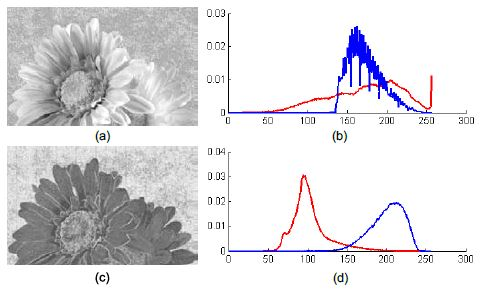
\includegraphics[width=0.8\columnwidth]{Chapter2/2/texture_figure_1.jpg}
\caption[Colour and texture image colour distributions.]{Intensity image with overlapping intensity distributions (top) and texture image with intensity distributions separated (bottom). Figure taken from \cite{texture}.}
\label{fig:texture-f1}
\end{figure}

\begin{figure}[t!]
\centering
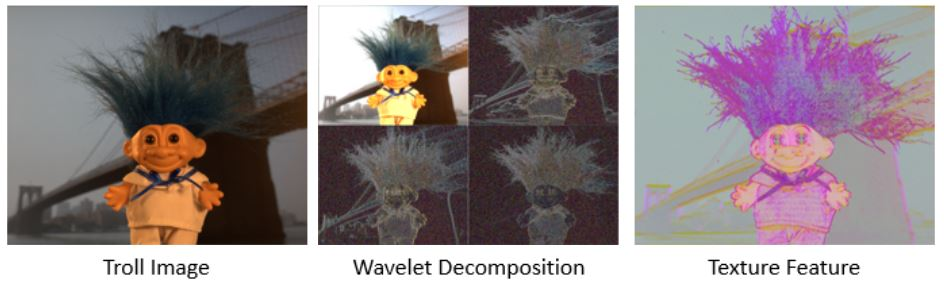
\includegraphics[width=1\columnwidth]{Chapter2/2/texture_figure_2.jpg}
\caption[Haar wavelet decomposition and resulting texture image.]{Visual representation of \textit{Haar wavelet decomposition} and resulting texture image. Figure taken from \cite{texture}.}
\label{fig:texture-f2}
\end{figure}

Another contribution by the same researchers in association with \textit{Adobe Research}, was to solve the problem of sampling non-representative samples. This comprehensive sampling approach \cite{comprehensive}, separates the trimap known region in to sub regions that are activated iteratively for sampling. Basically the more spatially close the samples are, the less the colour variation, and the further away there are the more colour variation is needed. This idea is illustrated in Figure 18. For selection of the best foreground and background sample pair, chromatic distortion \textit{K}, and spatial \textit{S} and colour \textit{C} statistics are considered (\ref{eq:comprehensive_e1}). The matte is further refined using the laplacian proposed in \cite{closedform}.

\begin{equation} \label{eq:comprehensive_e1}
O_{z}(F_{i},B_{i})=K_{z}(F_{i},B_{i})\times S_{z}(F_{i},B_{i})\times C_{z}(F_{i},B_{i})
\end{equation}

\begin{figure}[t!]
\centering
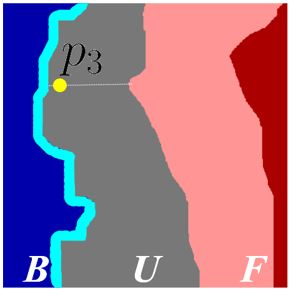
\includegraphics[width=0.4\columnwidth]{Chapter2/2/comprehensive_figure_1.jpg}
\caption[Comprehensive matting sampling strategy.]{\textit{Improving Image Matting Using Comprehensive Sampling Sets} sampling strategy. A pixel in unknown region (grey) samples from the activated foreground region (light blue), and from activated background region (light red). Figure taken from \cite{comprehensive}.}
\label{fig:comprehensive-f1}
\end{figure}

%%%%%%%%%%%%%%%%%%%%%%%%%%%%%%%%%%%%%%%%%%%%%%%%%%%%%%%%%%%%%%%%%%%%%%%%%%%%%%%%%%%55
\section{Extention to video}
\label{sec:extention-to-video}

Since the introduction of the blue screen matting technique, video matting has been increasingly used in the industry. Consequently research has also been focused to extend natural image mating to matting of natural video scenes. The basic challenges in video matting is the large data set, so algorithms must be fast enough to compensate for it, temporal coherence of frames, because the human visual system is sensitive to temporal inconsistencies, and fast motions that cannot be caught by the typical 30 frames per second that cameras capture, that cause motion blur. Because it would be impossible to define trimaps for every single frame manually, typical methods for introducing prior information is to define trimaps in key frames and interpolate the rest, by using \textit{optical flow} algorithms or use hard segmentation algorithms that are temporally consistent. Tracking algorithms that are used in computer vision for background removal, unfortunately cannot be used in matting because results of such methods are too coarse and not accurate enough either to generate a trimap or to give information to be used directly in a matting algorithm.
\par
The first video matting algorithm \cite{video} was based on Bayesian matting \cite{bayesian} and used with optical flow for temporal coherence. Trimaps were created by interpolating between keyframe trimaps provided by the user or automatically generated. Optical flow algorithms are used to estimate pixel motion in a video sequence. Assuming that we have two sequential frames, each pixel in one of the frames can be considered to be coming from a shifted location in the other frame, and the displacement of the pixel is described by a \textit{motion vector} and the set of motion vectors is called \textit{flow field} (Figure 19). Assumptions to be made are that the colour of the pixels is considered to estimate the flow field and a flow field should be spatially coherent. Many optical flow algorithms exist in the literature and for this video matting method an algorithm described in \cite{flow} is used. Sequential video frames are used to model a background using image mosaicking techniques \cite{mosaic} that can be used in cases where the background isn’t static to further refine the trimaps, assuming that the background in the video is roughly planar. Figure 20 illustrates the whole process.

\begin{figure}[t!]
\centering
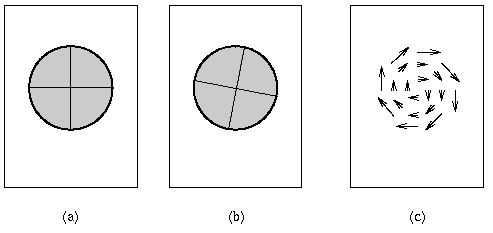
\includegraphics[width=0.8\columnwidth]{Chapter2/2/optical_figure_1.jpg}
\caption[Motion vectors and flow field.]{Two sequential frames at times t (a) and t+1 (b) and the estimated flow field (c). The arrows represent the motion vectors. }
\label{fig:optical-f1}
\end{figure}

\begin{figure}[t!]
\centering
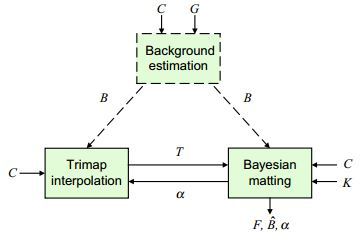
\includegraphics[width=0.8\columnwidth]{Chapter2/2/optical_figure_2.jpg}
\caption[Video matting work-flow.]{Work flow of the video matting algorithm. C is the frame sequence, G is the garbage mattes provided by the user, B is the estimated background, T is the trimap, a is the alpha mattes and K is the user provided keyframe trimaps. Figure taken from \cite{video}.}
\label{fig:optical-f2}
\end{figure}

%%%%%%%%%%%%%%%%%%%%%%%%%%%%%%%%%%%%%%%%%%%%%%%%%%%%%%%%%%%%%%%%%%%%%%%%%%%%%%%%%%%%%%%
\section{Matting with custom hardware}
\label{sec:matting-with-custom-hardware}

Due to the under-constrained nature of the matting problem, user input must be provided in a form of a trimap or sparse scribbles. In video matting, we saw that frame to frame variations can be used as extra information to help with the matting process. Researches have considered in a number of occasions the use of specialized hardware that will provide extra information needed to solve the matting problem.
\par
In \textit{Defocus matting} \cite{defocus}, multiple synchronized video streams are caught using a multi-sensor camera. This camera consists of three components, a pinhole sensor that has a small aperture that creates a large depth of field and is nominally focused on the foreground, a foreground sensor that produces sharp images for objects that are close to the camera and a defocused background, and a background sensor with a large depth of field (Figure 21). A trimap is automatically created by examining the texture of the images, specifically the sharp pixels correspond to the foreground for the foreground focused image and sharp pixels correspond to background for the background focused image. The disadvantages of this method is that the system requires a significant discontinuity between foreground and background and also the system requires stronger illumination than a normal camera.

\begin{figure}[t!]
\centering
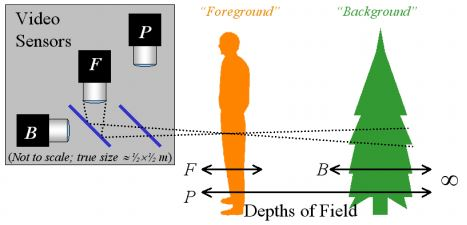
\includegraphics[width=0.9\columnwidth]{Chapter2/2/defocus_figure_1.jpg}
\caption[Defocus matting setup.]{The multi-sensor camera system with a pinhole sensor P, a foreground focused camera F and a background focused camera B. Figure taken from \cite{defocus}.}
\label{fig:defocus-f1}
\end{figure}

In \textit{Flash matting} \cite{flash}, the idea is that when an object is photographed, the flash does not affect the background in a significant way. So if a scene if photographed with and without flash and then the two resulting images are subtracted, the result will be a rough foreground that can be used to produce a trimap. In a sense, this is the reverse process of triangulation \cite{blue}; instead of having two different backgrounds, we have two different foregrounds. The disadvantage of this method is that objects with specular properties may produce an erroneous trimap because the high reflectance areas will not change in the two images.

\begin{figure}[t!]
\centering
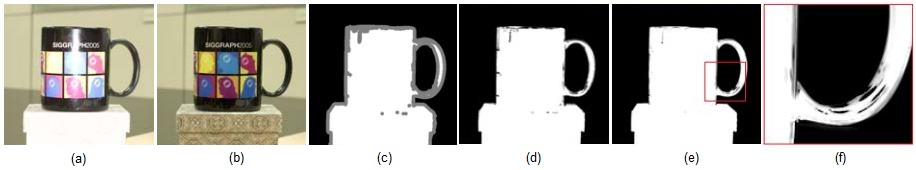
\includegraphics[width=1\columnwidth]{Chapter2/2/flash_figure_1.jpg}
\caption[Flash matting images and results.]{An object photographed with (a) and without (b) flash, the produced trimap (c), and the problematic areas due to specular surfaces. Figure taken from \cite{flash}.}
\label{fig:flash-f1}
\end{figure}

The next approach uses a \textit{camera array} \cite{cameraarray} to solve the matting problem. A synthetic image is created that is focused on the foreground object which reduces the variance of the pixels in the foreground and increases the variance of pixels in the background. The standard matting equation is modified to work with the variances of the images. So basically the foreground is captured in front of multiple backgrounds, created by the parallax of the images. This system has shown good results on a variety of images containing fuzzy and transparent regions and is also quite fast with running times close to real time for VGA images. The drawback though is that the accuracy is limited by aliasing in the light fields and the fact that the system is designed to work better in controlled environments that are usually indoor.
\par
A recent tendency in computer vision is the use of depth information produced by \textit{time of flight} TOF sensors. These sensors are able to produce high quality \textit{depth-maps} that can be further used in the matting process. A depth-map is known to be used for z-buffering in computer graphics, but has many application in computer vision. Extracting depth information from images only is a difficult process, so the use of a device that can provide the depth-map is preferred. In \cite{tof} the authors are using a time of flight sensor in combination with a stereo rig. They first create an initial matte that is extracted from the depth-map produced by the TOF sensor and then the matte and depth are refined. A trimap is created by use of erosion and dilation techniques on the extracted depth and the closed form method \cite{closedform} is used to produce the initial matte. In the refinement phase a cost function is created by using depth, pixel similarity from stereo matching and the confidence from the matte. Figure 23 illustrates the mattes and depth-maps produced.

\begin{figure}[t!]
\centering
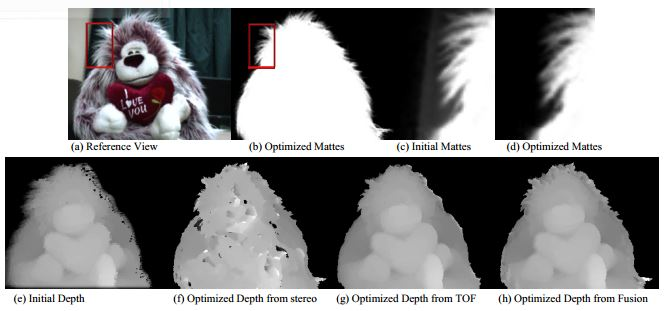
\includegraphics[width=0.8\columnwidth]{Chapter2/2/depth_figure_1.jpg}
\caption[Matting with depth information.]{Estimated alpha matte (b), depth-map (h) and optimizations. Figure taken from \cite{tof}.}
\label{fig:depth-f1}
\end{figure}

An extension of this method in \cite{realtimetof} proposes an automatic real-time video matting system. The system is initialized by using colour and depth information. The hard segmentation is done by modelling foreground, background colours and depth likelihoods and by using \textit{graph cuts}. From the binary mask produced from the hard segmentation, a trimap is generated and refined using the colour and depth information and then the final matte is estimated using multichannel Poisson equations. The algorithm is implemented on GPU and for a low resolution image the hard segmentation implementation can achieve 32fps and the matting implementation archives 80fps. The limitation of this system is that the hard segmentation process is done frame by frame and no temporal coherence is enforced for the trimaps. Figure 24 illustrates the work flow.

\begin{figure}[t!]
\centering
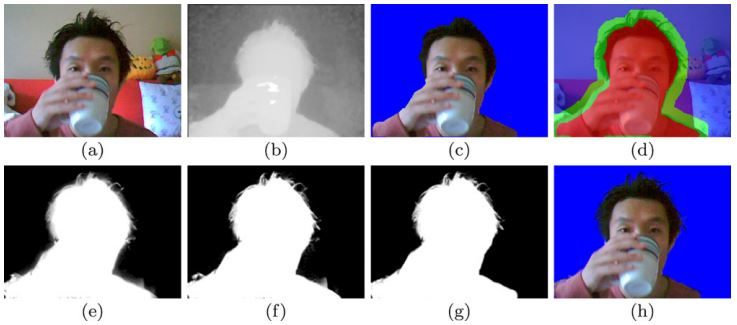
\includegraphics[width=0.8\columnwidth]{Chapter2/2/depth_figure_2.jpg}
\caption[Real-time matting with depth.]{From a colour image (a) and a depth-map (b), a binary mask (c) is produced and refined into a trimap (d). The alpha matte is iteratively produced (e)(f)(g)(h). Figure taken from \cite{realtimetof}.}
\label{fig:depth-f2}
\end{figure}


\chapter{Development tools}
\label{sec:development-tools}

For experimental work and implementation purposes we used the Kinect SDK in combination with EMGU (C\#) and OpenNI combined with OpenCV (C++). The Kinect SDK and OpenNI were used to capture colour and depth images from the Kinect sensor. The initial preliminary work for basic foreground extraction was done using the computer vision library EMGU and the Kinect SDK. The majority of the experimental work that was done later on, was implemented in OpenCV because it provided more features, more openness and better flexibility in programming.

\section{OpenCV}
\label{sec:opencv}

\textit{OpenCV} is an open source library consisting of computer vision algorithms, and was originally developed by \textit{Intel} and is now supported by \textit{Willow Garage} and \textit{Itseez}. OpenCV consists of libraries mainly for C/C++ development and interfaces are also provided for Python, Java and Matlab. EMGU is a wrapper of OpenCV libraries and is used for .Net development. Part of the OpenCV framework are CUDA and OpenCL based GPU interfaces. The basic structure of OpenCV is the core module that contains methods for data structure definition and matrix manipulation, the image processing module that includes various image processing algorithms, the interface module that offers image and video loading and presenting capabilities, the feature description and detection module, the machine learning module and other computer vision related modules that are useful for application or experimental development.

\section{Kinect}
\label{sec:kinect}

The Kinect sensor is a consumer grade imaging device developed by \textit{Microsoft} in 2010 to be used as a natural interaction medium for computer game environments, with original development by Israeli company \textit{PrimeSence}. Its low cost, though, along with its range sensing capabilities has attracted the attention of researchers and computer vision enthusiasts. The Kinect sensor can produce depth and colour streams simultaneously at a frame rate of 30 fps with resolutions 640X480. The colour stream is also scaled to 1280X960 resolution at 15 fps. The sensor consists of an infrared laser emitter, an infrared camera and an RGB camera. The depth is measured by a triangulation process, where the laser emits a beam that is split into multiple beams by a diffraction grating to create a constant pattern of speckles projected onto the scene \cite{kinectaccuracy}. The produced pattern is captured by the infrared camera and correlated against a reference pattern to estimate depth. This method for extracting depth information is also known as \textit{structured light scanning} \cite{kinectaccuracy}. The depth measurement is in millimetres and depth sensing ranges from 400mm to 8000mm (Figure \ref{fig:depth-dist}).

\section{Kinect SDK and OpenNI}
\label{sec:openni}

The original Kinect was released for the Xbox 360 in 2010 and a Windows version for development purposes was released later on along with the Kinect SDK in 2012. The Kinect SDK has a core module called Natural User Interface that handles colour and depth streams, player and skeletal tracking and audio streams, a module for gesture recognition, the Kinect Fusion module that deals with 3D reconstruction, a face tracking module, a back removal module and a module for web application development. The Natural User Interface module handles the depth stream in different resolutions and formats. As mentioned previously, the depth measures from 400mm to 8000mm but the recommended values are the ones between 800mm and 4000mm; distances further than 4000mm are considered too far and distances closer than 800mm are considered too near (Figure \ref{fig:depth-dist}). Flags can be set for the desired depth stream distances to be used.
\par
\textit{OpenNI} is a framework that contains open source drivers and APIs that provide tools for gesture recognition, body motion tracking and other natural interaction interfaces. It is supported mainly by PrimeSence and Asus, that have developed their own range sensing devices, and Willow Garage, a computer vision and robotics research centre. PrimeSence has been acquired by Apple in 2013 and subsequently in April 2014 OpenNI website was shut down. Forks of older versions of the framework can still be found online. Unfortunately the components of OpenNI are limited to basic stream acquisition, skeletal and hand tracking and some other features, since the more advanced features were part of Nite that was developed by Primesence and now is not available.

\begin{figure}[t!]
\centering
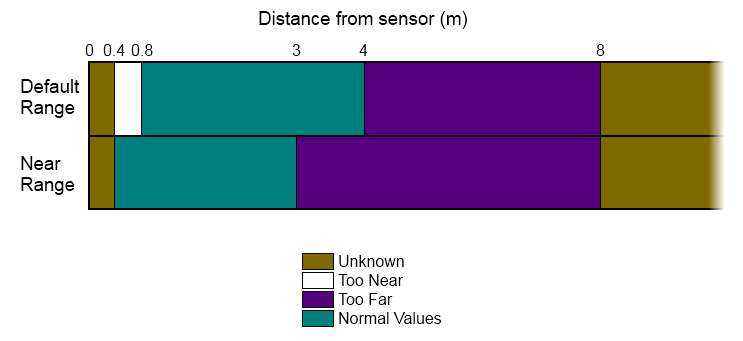
\includegraphics[width=1\columnwidth]{Chapter3/3/depth_dist.png}
\caption[Depth stream distances.]{The Kinect SDK handles the depth stream by separating the distances in to categories that the developer can choose from depending on the application.}
\label{fig:depth-dist}
\end{figure}
\chapter{Preliminary work}
\label{sec:preliminary-work}

\section{Basic hard segmentation}
\label{sec:basic-segmentation}

The first attempt for foreground extraction was done by using segmentation algorithms \textit{Watershed} \cite{watershed} and \textit{GrabCut} \cite{grabcut} and by using basic thresholding and filtering on the Kinect depth-map.
\par
The Kinect depth-map values are thresholded based on a pre-set maximum depth in order to get a rough estimation of the foreground (Figure \ref{fig:depth-pre-f}b). Because the result though cannot be used directly due to noise in the depth-map, the thresholded depth-map was preprocessed using a blurring filter. Then a binary threshold operation was used, to convert all the foreground values to a single one in order to create a binary mask (Figure \ref{fig:depth-pre-f}c) that was further used to map the pixels in the colour image (Figure \ref{fig:results-pre-f}b).
\par
A Watershed segmentation algorithm takes the gradient of the grayscale image and considers high intensities as maxima and low intensities as minima. Maxima and minima form "valleys" and "peaks" in an image and by using a flooding technique valleys are flooded and to avoid valleys from being connected, "walls" are built on the boundaries and at the end of the process those walls produce the segmented image. Image that has many valleys/peaks and noise would produce many such walls, resulting in a bad segmentation, so usually markers are introduced to define which valleys to be merged for a better segmentation results (Figure \ref{fig:water-f}). In our case, the binary mask that was calculated in the previous method, was used as a marker parameter in the OpenCV function watershed. To create the marker parameter, the binary mask was \textit{eroded} and \textit{dilated} and then the results of these operations were combined in order to mark the boundaries of the foreground region that would be segmented by the watershed algorithm (Figure \ref{fig:depth-pre-f}d). Erosion and dilation are morphological operators that process images based on shapes within them. A kernel is used in order to remove or add boundary pixels around a shape in an image (Figure \ref{fig:dilation-f}). The kernel is usually a 3x3 cross but others can be used, and the centre pixel serves as an anchor point on the shape boundary such that the rest of the pixels in the kernel denote whether pixels should be added or removed depending on the operation. The magnitude of the operations is set based on the iterations the process runs.

\begin{figure}[t]
\centering
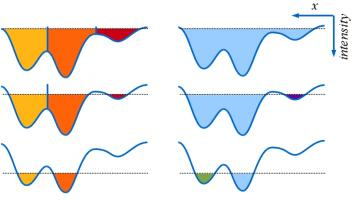
\includegraphics[width=0.7\columnwidth]{Chapter4/4/watershed.jpg}
\caption[Watershed flooding algorithm illustration.]{\textit{Watershed} flooding algorithm illustration. Valleys are flooded and "walls" are built in order to separate the regions (left). The user can specify valleys that are considered similar or noise to be connected during the flooding process (right).}
\label{fig:water-f}
\end{figure}

\begin{figure}[t]
\centering
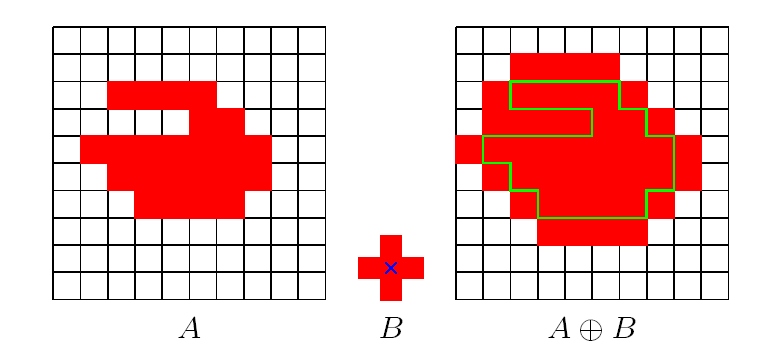
\includegraphics[width=0.8\columnwidth]{Chapter4/4/dilation.png}
\caption[Dilation on a binary image.]{\textit{Dilation} is a moprhological operator that uses a kernel to add pixels on a shape boundaries. The blue cross denotes the anchor point with the shape boundary and the rest of the pixels in the kernel denote pixels to be added.}
\label{fig:dilation-f}
\end{figure}

\par
Grabcut is a segmentation tool developed by Microsoft Research in 2004. The user specifies a bounding box around the object to be segmented (Figure \ref{fig:grab-f}) and and the colour distributions of the object and the background are modelled as Gaussian Mixture models based on the fact that everything outside the box is definite background. A graph is build based on the distributions where foreground and background nodes are connected to their corresponding foreground and background super-nodes and by using an energy minimization approach and iterated graph cuts, the foreground is hard segmented (Figure \ref{fig:graph-f}). The method has further optimizations where a user can denote with scribbles erroneously classified regions (Figure \ref{fig:grab-f}) and the process re-runs with this additional information. GrabCut has also a border matting component that softens the segmented object's boundary. In order to automate the process we took the binary mask generated from the depth-map, found the largest contour in the image using OpenCV findContour, then based on that contour we found the minimum and maximum coordinates from left to right and top to bottom and used them to create a bounding box around the foreground (Figure \ref{fig:depth-pre-f}d). Then we passed it to OpenCV's grabcut function along with the colour image to get the segmentation result.

\begin{figure}[t]
\centering
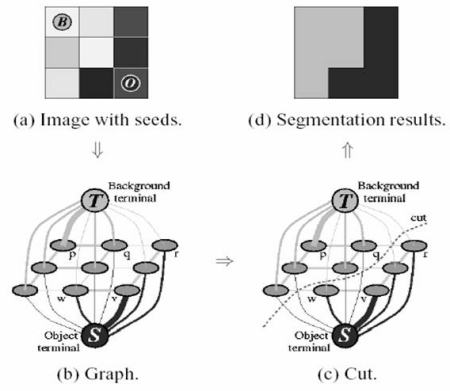
\includegraphics[width=0.6\columnwidth]{Chapter4/4/graphcut.jpg}
\caption[Graph cuts segmentation.]{\textit{GrabCut} uses graph cuts in-order to segment the image. Figure taken from \cite{grabcut}.}
\label{fig:graph-f}
\end{figure}

\begin{figure}[t]
\centering
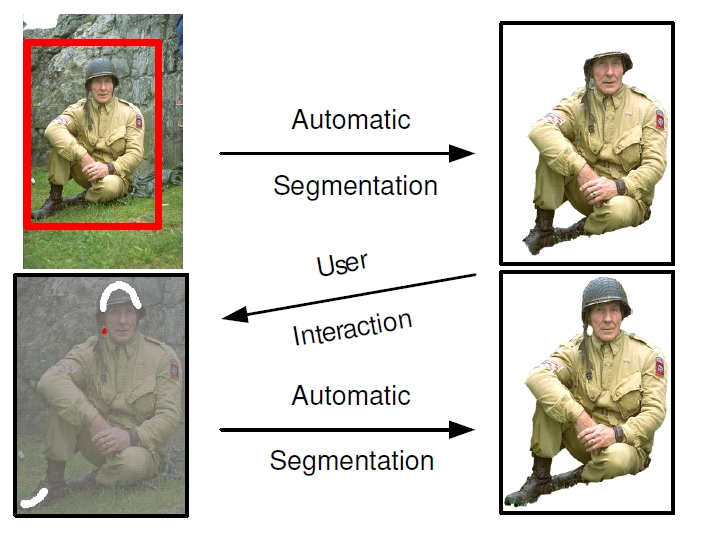
\includegraphics[width=0.6\columnwidth]{Chapter4/4/grabcut.png}
\caption[GrabCut example.]{\textit{GrabCut} has a simple interface for foreground extraction but usually need additional user input to get a good result. The user specifies a bounding box around the object to be segmented and then provides scribbles on erroneous regions as additional input. Figure taken from \cite{grabcut}.}
\label{fig:grab-f}
\end{figure}

\par
The results in general were not acceptable, even in images with a simple background (Figure \ref{fig:results-pre-f}). This was primary due to the fact that the depth-map contained too many errors, the watershed algorithm could not segment the image correctly based on the markers provided, and the grabcut algorithm needed additional user input in order to fix the erroneous regions.

\begin{figure}[t]
\centering
\subfloat[][Thresholded depth]{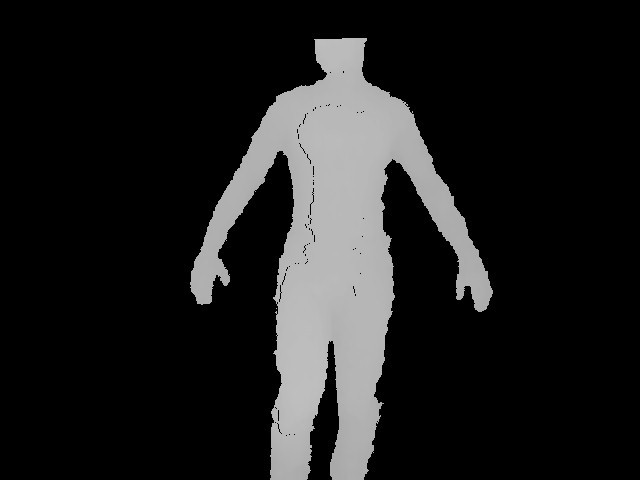
\includegraphics[width=0.4\columnwidth]{Chapter4/4/depth.jpg}}
\subfloat[][Binary mask]{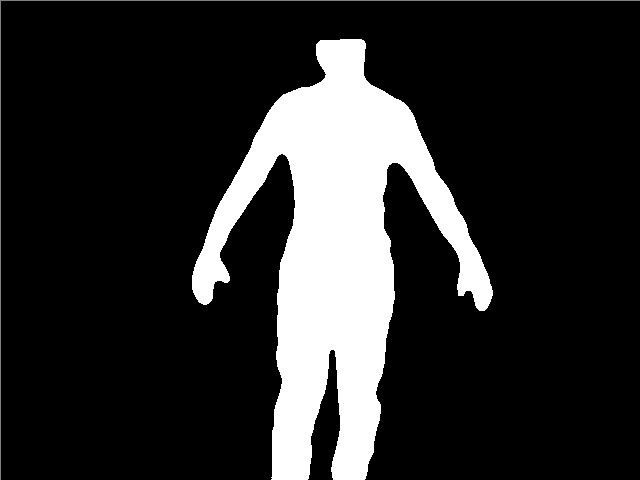
\includegraphics[width=0.4\columnwidth]{Chapter4/4/binary.jpg}}
\newline
\centering
\subfloat[][Markers]{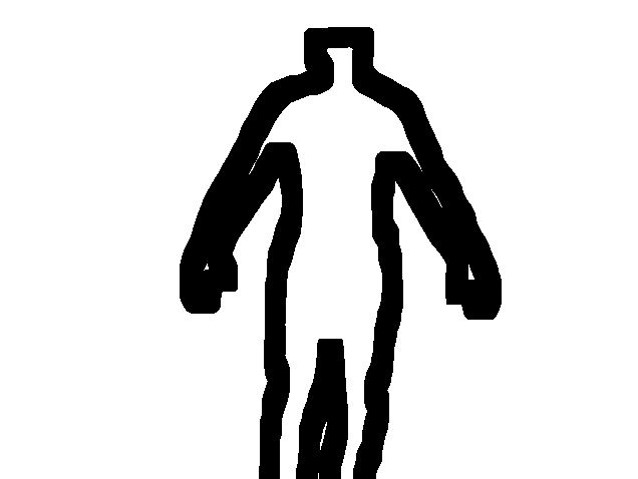
\includegraphics[width=0.4\columnwidth]{Chapter4/4/markers.jpg}}
\subfloat[][Bounding box]{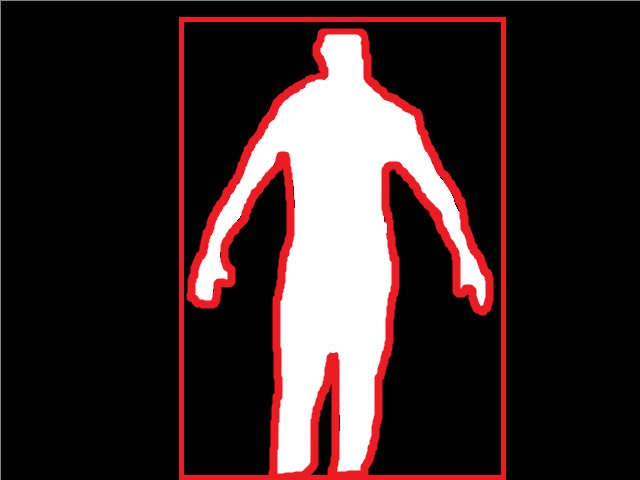
\includegraphics[width=0.4\columnwidth]{Chapter4/4/depth_box.jpg}}
\caption[Depth-map pre-processing for various methods.]{Depth-map pre-processing for various methods. A binary mask is generated from the thresholded depth to be used for compositing. The binary mask is further used to create markers for the Watershed method and to create a bounding box for the GrabCut method.}
\label{fig:depth-pre-f}
\end{figure}

\begin{figure}[t]
\centering
\subfloat[][RGB image]{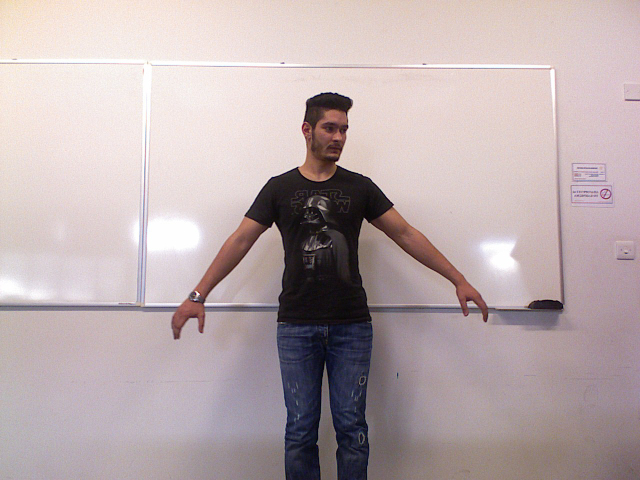
\includegraphics[width=0.4\columnwidth]{Chapter4/4/image1.jpg}}
\subfloat[][Depth-map bluring result]{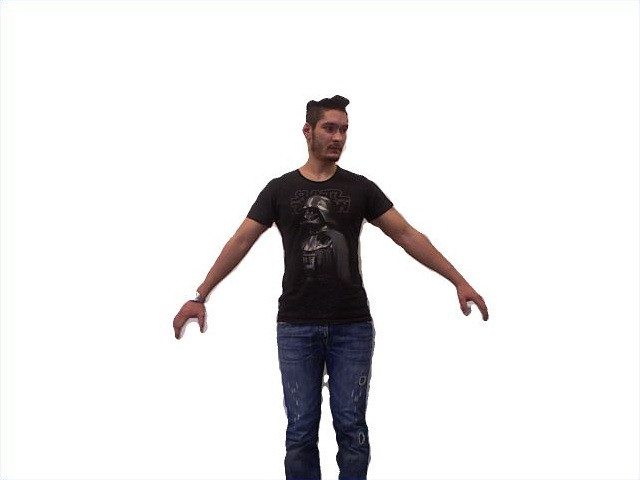
\includegraphics[width=0.4\columnwidth]{Chapter4/4/blur1.jpg}}
\newline
\centering
\subfloat[][Watershed result]{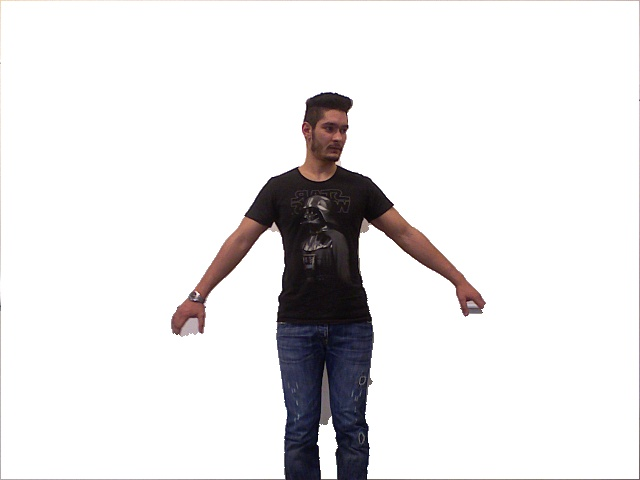
\includegraphics[width=0.4\columnwidth]{Chapter4/4/water1.jpg}}
\subfloat[][GrabCut result]{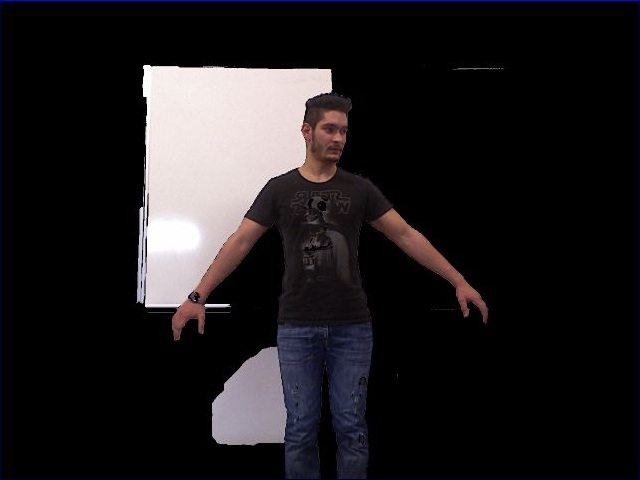
\includegraphics[width=0.4\columnwidth]{Chapter4/4/grab1.jpg}}
\caption[Results from various segmentation methods.]{Results from crating a binary mask from the depth-map (b) and from segmentation methods Watershed (c) and GrabCut (d).}
\label{fig:results-pre-f}
\end{figure}

%%%%%%%%%%%%%%%%%%%%%%%%%%%%%%%%%%%%%%%%%%%%%%%%%%%%%%%%%%5
\section{Machine learning segmentation}
\label{sec:learning-segmentation}

The next attempt was a manual approach to segmentation, were machine learning algorithms \textit{K-Nearest Neighbours} and \textit{Support Vector Machines} were used to classify pixels into foreground and background.
By providing a machine learning algorithm with foreground and background samples and their corresponding classes, pixels could be classified into foreground or background class and the result would eventually be a binary mask.
\par
The K-Nearest Neighbour algorithm is a supervised learning algorithm. Assume that we have a set of multiple items. Each item is labelled and belongs to a certain class. When a new item is added to the set it is labelled according to its similarity with the other items. This similarity is measured by its distance from the other items in a feature space. For example, in Figure \ref{fig:knn-space-f} the new item (in green) is classified based on its distance from the other items. The value of K is crucial for classification, since as illustrated in the Figure \ref{fig:knn-space-f}, two different values of K produce different classification results. The number K should always be odd in order to avoid ties.

\begin{figure}[t]
\centering
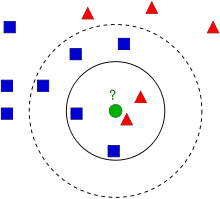
\includegraphics[width=0.5\columnwidth]{Chapter4/4/knn.png}
\caption[KNN 2-D sample space visualization.]{In \textit{K-Nearest Neighbours}, when a new item is added to the set, it is classified based on the K nearest samples to it.}
\label{fig:knn-space-f}
\end{figure}

Support vector machines is also a non-probabilistic supervised learning algorithm. Assuming again that we have a set of items, they are separated into classes using a hyperplane. The optimal hyperplane is the one that separates the items by having a maximum margin from all of them (Figure \ref{fig:svm-space-f}). Since data cannot always be separated linearly, an extension to the algorithm re-classifies misclassified items by considering the distance of items from the outer margin of the hyperplane.

\begin{figure}[t]
\centering
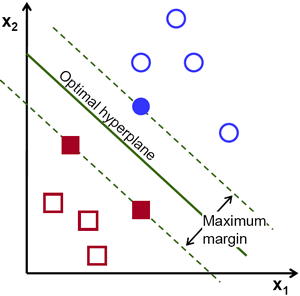
\includegraphics[width=0.5\columnwidth]{Chapter4/4/svm.png}
\caption[SVM 2-D sample space visualization.]{In \textit{Support Vector Machines}, a line that is considered the hyperplane in 2D space, optimally separates the data by considering the largest possible margin between sample sets.}
\label{fig:svm-space-f}
\end{figure}

In order to be able to provide training samples to the machine learning algorithms, we needed to create a trimap that would contain definite foreground, definite background and unknown regions. This was done by using the binary mask that had been produced in previous methods. The binary mask was eroded and dilated and the resulting masks were combined in-order to create a trimap. The basic sampling strategy was to take all the foreground and all the background pixels as training sets, but this would contribute to high running times. To solve this problem we created a new trimap that had two extra regions that were created by eroding and dilating the binary mask with a higher magnitude this time and by adding the previous masks with the two new ones to create a five-region map. Initially, all the pixels in the two extra regions were sampled to be used for training purposes and RGB values were used as features. 
\par
OpenCV includes a machine learning module that has implementations of KNN and SVM, and were used for the classification process. We provided them with the training sample sets and their corresponding classes in order to train the algorithms, and then iterated for each unknown pixel to classify it. The results weren't satisfactory and running times were still high, so by assuming that pixels close to each other have similar attributes, we used a local sampling approach by sampling pixels within a circle around the unknown pixel (Figure \ref{fig:old-method-f}). By sampling N random samples within the circle instead of all, we managed to reduce running times even more.
Tests were run with global and local sampling, on images with various foregrounds and backgrounds and the best approach was local sampling with KNN (Figure \ref{fig:results-machine-f}b). SVM failed to classify many of the unknown pixels even with an easy background (Figure \ref{fig:results-machine-f}a). KNN failed to correctly classify pixels in images with a difficult background (Figure \ref{fig:results-machine-f}d).

\begin{algorithm}
\caption{Sampling K random samples within a circle.}\label{old-sampling-method}
\begin{algorithmic}[1]
\ForAll{unknown pixels}
\ForAll{foreground and background pixels in circle}
\State F sample set $\gets$ get N random foreground samples
\State B sample set $\gets$ get N random foreground samples
\EndFor
\EndFor
\State Classification
\end{algorithmic}
\end{algorithm}

\begin{figure}[t!]
\centering
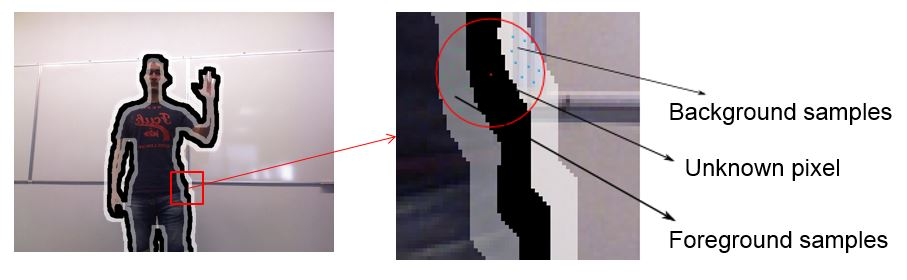
\includegraphics[width=1\columnwidth]{Chapter4/4/old_method.jpg}
\caption[Old sampling strategy.]{Five region map and sampling scheme. The five region map was an extension of the trimap that has two additional regions used for sampling. The sampling was done by selecting random samples within a radius around the unknown pixel.}
\label{fig:old-method-f}
\end{figure}

\begin{figure}[t]
%\centering
\subfloat[][SVM result]{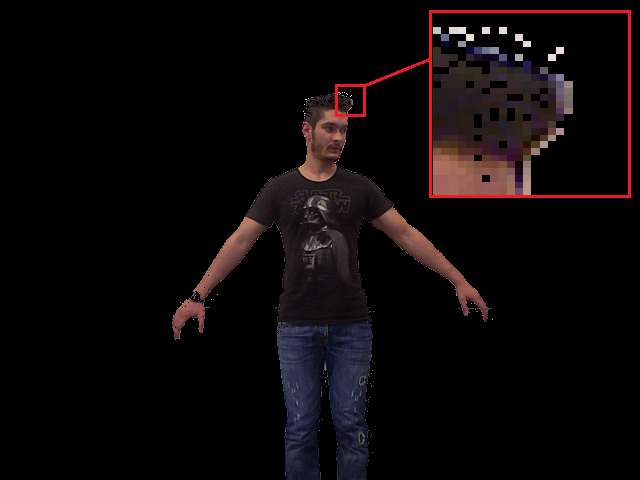
\includegraphics[width=0.5\columnwidth]{Chapter4/4/local_nonlinear_svm__result2.png}}
\subfloat[][KNN result]{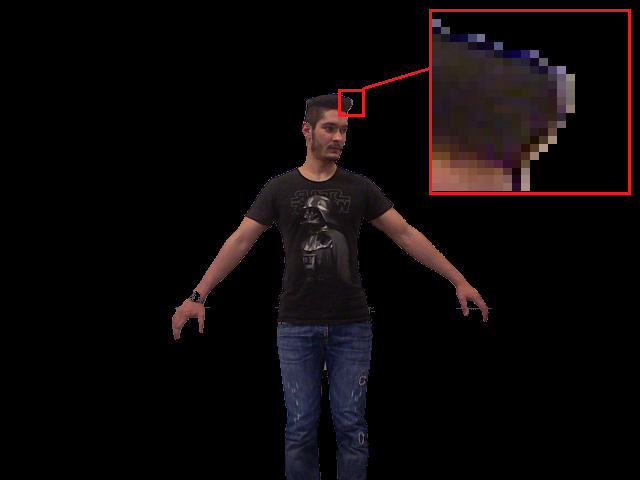
\includegraphics[width=0.5\columnwidth]{Chapter4/4/local_random_knn.png}}
\newline
\subfloat[][RGB image]{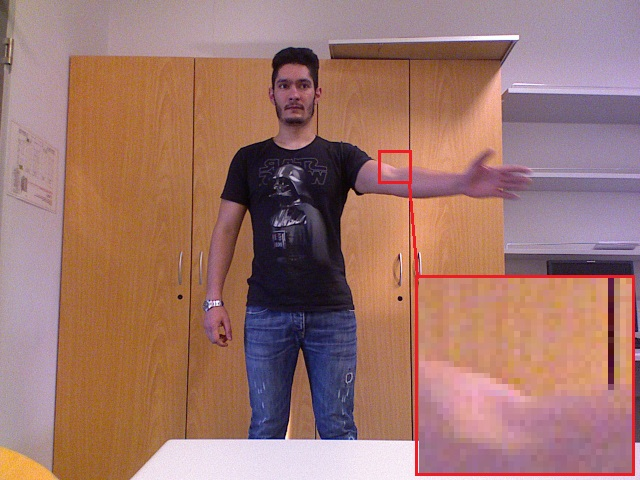
\includegraphics[width=0.5\columnwidth]{Chapter4/4/image2.png}}
\subfloat[][KNN result]{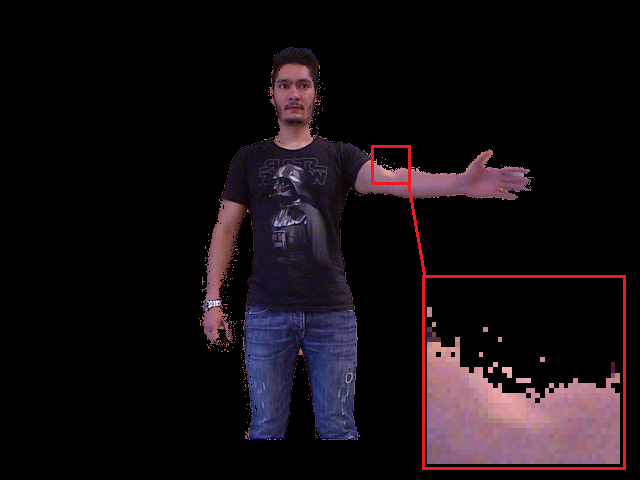
\includegraphics[width=0.5\columnwidth]{Chapter4/4/local2_random_knn.png}}
\caption[Results from machine learning based segmentation.]{For both methods sampling is local and KNN produces a better segmentation result than SVM. For a difficult background though, the KNN fails to classify many pixels resulting in a noisy boundary.}
\label{fig:results-machine-f}
\end{figure}

%%%%%%%%%%%%%%%%%%%%%%%%%%%%%%%%%%%%%%%%%%%%%%%%%%%%%%%%%%%%%%%%
\section{Early alpha matting}
\label{sec:early-matting}

At this point we considered using the matting equation that could produce the fuzzy alpha values that give a better representation of the mixed pixels in the image. In images taken from the Kinect, these kind of pixels were usually found in the boundaries of the foreground.
The matting equation requires a foreground value, a background value and the unknown pixel value in order to produce the $\alpha$ value. Since our previous approach classified a pixel into a certain class and didn't return the values of the best matching foreground and background pixels, we devised a pixel differencing method that returned the best foreground and background values that were needed to produce the $\alpha$ values.
Similarly to KNN, we formed a feature vector for each pixel that consisted of colour and spatial information, and each of the foreground and background samples feature vectors were differenced with each unknown pixel feature vector. From each of the foreground and background distance sets the K smallest differences where selected and were thereafter averaged to get the final values that would be used in the matting equation for $\alpha$ estimation.

\begin{algorithm}
\caption{Pixel differencing and averaging of best foreground and background samples.}\label{differencing-method}
\begin{algorithmic}[1]
\State Sampling
\ForAll{unknown pixels}
\ForAll{foreground samples}
\State distances set $\gets$ Difference(F, U)
\Comment{Absolute value of difference}
\EndFor
\State K smallest set $\gets$ GetSmallest(distances set)
\State F $\gets$ Average(K smallest set)
\ForAll{background samples}
\State distance set $\gets$ Difference(B, U)
\Comment{Absolute value of difference}
\EndFor
\State K smallest set $\gets$ GetSmallest(distances set)
\State B $\gets$ Average(K smallest set)
\EndFor
\end{algorithmic}
\end{algorithm}

For problematic regions with overlapping colour distributions we used \textit{Local Binary Patterns} \cite{lbp} as an extra feature. Local binary patterns are binary codes that represent a pixels texture. Figure \ref{fig:lbp-m-f} illustrates the process for computing the LBPs. The results weren’t improved mainly due to the fact that LBP provide general information about an image texture, usually via a histogram, and not pixel based information, LBPs failed to separate regions with similar colours but different texture (Figure \ref{fig:lbp-f}).

\begin{figure}[t]
\centering
\includegraphics[width=0.8\columnwidth]{Chapter4/4/lbp.jpg}
\caption[Local binary patterns computation methodology.]{\textit{Local binary patterns} are computed on the grayscale image.}
\label{fig:lbp-m-f}
\end{figure}

\begin{figure}[t]
\centering
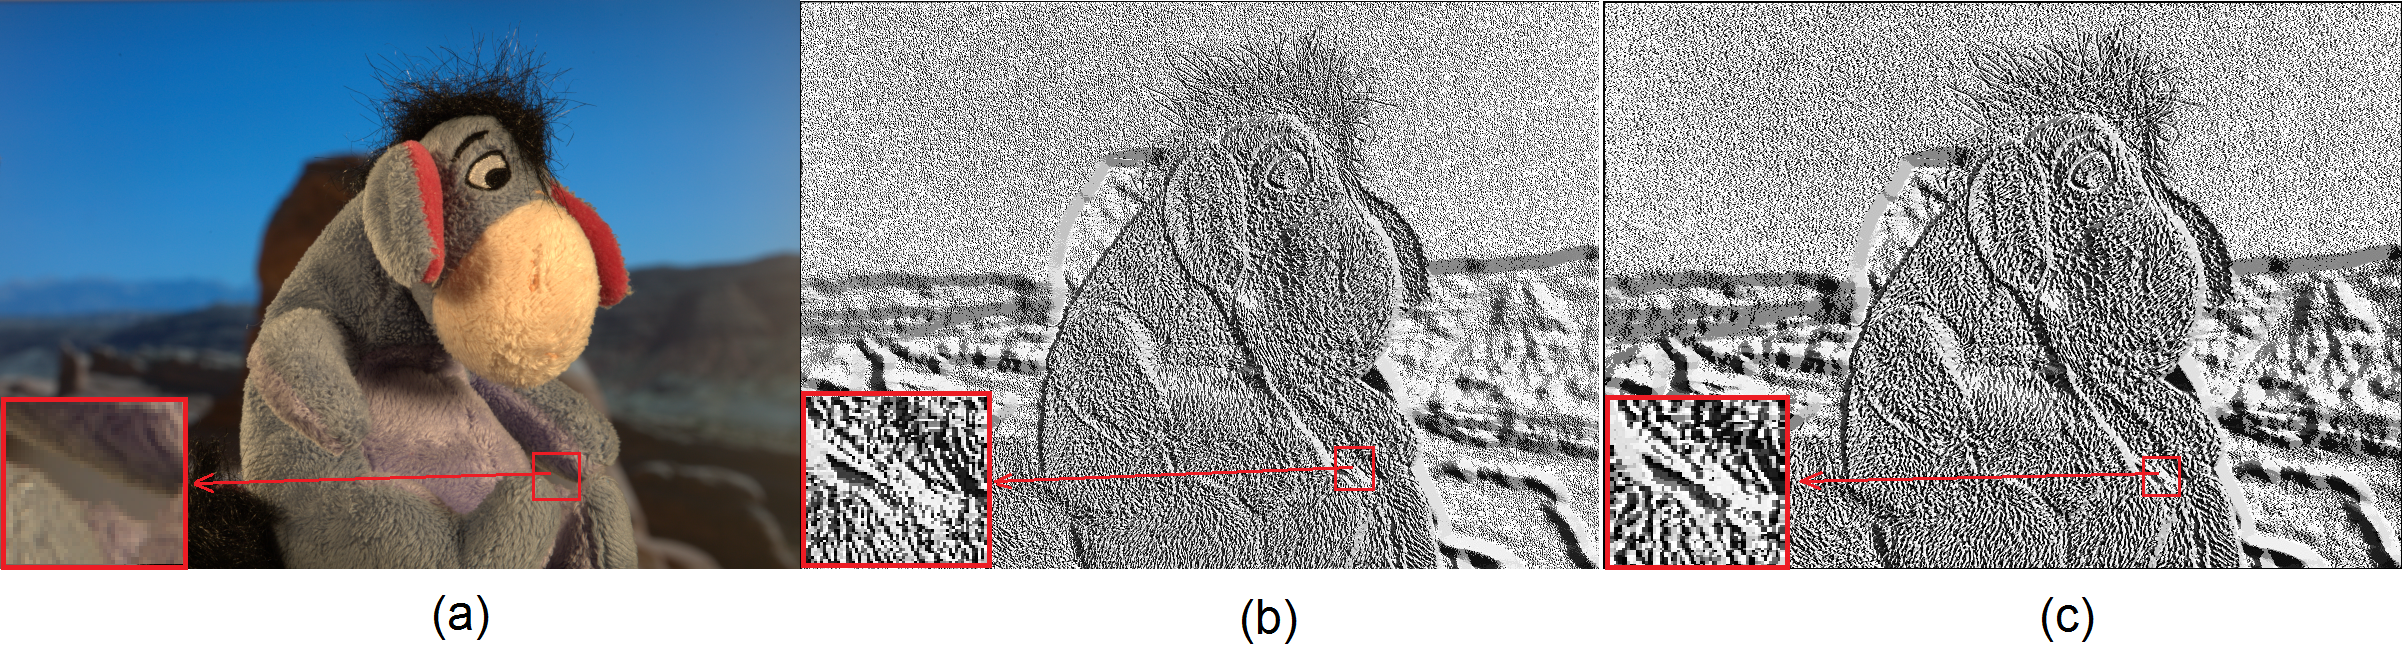
\includegraphics[width=1\columnwidth]{Chapter4/4/lbp_figure.jpg}
\caption[Local binary patterns visualization.]{Local binary patterns images, produced by an 8x8 window (b) and 16x16 window (c). LBP fails to separate regions with similar colours but different texture in the image version of them.}
\label{fig:lbp-f}
\end{figure}

Since LBP did not solve the problem of overlapping F and B colour distributions, we re-assessed the problem and observed that colour images taken from the Kinect, had colour distortion due to jpeg compression and this contributed to the problem of miss-classified pixels. To tackle this issue we used the \textit{Kuwahara filter} that is an noise reducing, edge preserving filter. The Kuwahara filtering algorithm uses sliding window over each pixel and uses the variance of the mean of surrounding pixel regions in order to determine the value of the centre pixel. For colour images the variance is determined from the brightness channel of the HSV colour space and the colour channel values are determined by the mean the pixels in the region with the least variance for each colour channel.
This preprocessing work helped reduce miss-classified pixels that were far from from their corresponding region but it produced some artifacts on the edges of the foreground that caused misclassification of other pixels. Also the Kuwahara filter is a non-linear filter that produced an overhead in running times for high resolution images.

\begin{figure}[t]
\centering
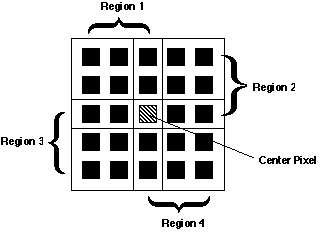
\includegraphics[width=0.6\columnwidth]{Chapter4/4/kuwa.png}
\caption[Kuwahara filter window illustration.]{The \textit{Kuwahara filter} uses a sliding window, where the centre pixel value is determined by the least variance of the mean of each pixel region.}
\label{fig:kuwahara-f}
\end{figure}

\begin{figure}[t]
\centering
\includegraphics[width=1\columnwidth]{Chapter4/4/Kuwahara_figure.jpg}
\caption[Kuwahara filter example.]{The \textit{Kuwahara filter} has noise reduction and edge preserving properties.}
\label{fig:kuwahara-f}
\end{figure}

For smoothness, we used a feature that was derived from a mask that weighted unknown region values based on their distance from the foreground. The mask was created by applying a blurring filter to the binary mask (Figure \ref{fig:blur-weight-f}). The values were normalized before use and their magnitude was downgraded so they would not dominate in the feature space. The kernel size for the blurring filter was chosen to produce a blurred region that would be as wide as the unknown region. This approach worked well in cases were the total unknown region had a smooth width around the foreground region.

\begin{figure}[t]
\centering
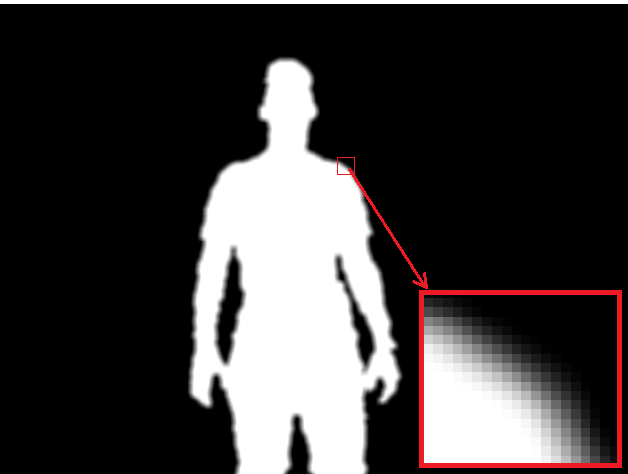
\includegraphics[width=0.8\columnwidth]{Chapter4/4/blur_weight.png}
\caption[Mask that weights the unknown pixels based on their distance from the foreground.]{Mask that weights the unknown pixels based on their distance from the foreground.}
\label{fig:blur-weight-f}
\end{figure}
\chapter{Algorithm: Nearest sample matting}
\label{chap:nearest-sample-matting}

%\section{Introduction}
%\label{sec:introduction}

After reviewing various matting methods we noticed that each algorithm works best in specific cases and algorithms that work for all cases do not give satisfying results. The steps that formulate an algorithm that are common in all matting methods consist of getting the input data to be segmented either as an image or as a video frame, get the prior information either by user input or automatically using the methods described in Chapter 2, sample foreground and background pixels based on the prior information to create a training set of data that characterises the image background and foreground, and then select the best foreground and background samples in order to classify each unknown pixel into those two sets definitely or relatively based the matting equation so that an alpha matte is created. The last step is to refine the estimated alpha matte for smoothness. 

\begin{algorithm}
\caption{Matting methodology}\label{matting-method}
\begin{algorithmic}[1]
\State Get input image
\State Get trimap
\ForAll{unknown pixels}
\State Sample F and B
\State Get best F and B
\State Calculate $\alpha$
\EndFor
\State Refine alpha matte
\end{algorithmic}
\end{algorithm}

For the formulation of our own algorithm we considered the steps mentioned above and focused on getting an accurate matte using benchmark datasets and images produced by the Kinect sensor, without using refinement methods for smoothness or connectivity.

%%%%%%%%%%%%%%%%%%%%%%%%%%%%%%%%%%%%%%%%%%%%%%%%%%%%%%%%%%%%%%%%%%%%
\section{Sampling}
\label{sec:sampling}

The sampling procedure starts by iterating through each unknown pixel and for each one all the neighbouring pixels that belong to foreground and background are sampled within a small radius. The sampling radius around the unknown pixel grows until a specified amount of samples is gathered. This methodology samples the most spatially close pixels and according to other matting methods, pixels that are close to each other tend to share similar attributes and thus increase the probability of correct classification. For scribble based trimaps we used a global sampling approach, where all pixels in the definite foreground and definite background are used as samples. When using global sampling and the number of samples is too high, experiments on images with small fuzzy regions showed that sampling every other or every few pixels (50\%-20\% of total) reduces running time significantly with little affect on the resulting alpha matte quality .This again, is due to the fact that pixels that are close share similar attributes.

\begin{algorithm}
\caption{Sampling algorithm}\label{sampling-algorithm}
\begin{algorithmic}[1]
\ForAll{unknown pixels}
\While{$F\; set < min\; \textbf{OR}\; B\; set < min$}
\ForAll{pixels in radius R}
\State Add pixel to \textit{F set}
\State Add pixel to \textit{B set}
\EndFor
\State R $\gets$ R + 1
\EndWhile
\State Classification
\EndFor
\end{algorithmic}
\end{algorithm}

\begin{figure}[t!]
\centering
\includegraphics[width=1\columnwidth]{Chapter5/5/win.png}
\caption[Sampling radius.]{The sampling radius grows until a minimun number of F and B samples is gathered.}
\label{fig:window-f}
\end{figure}

\begin{figure}[t!]
\centering
\includegraphics[width=1\columnwidth]{Chapter5/5/sampling_window.jpg}
\caption[New sampling strategy.]{Sampling strategy that gathers all the pixels within a window around an unknown pixel.}
\label{fig:sampling-window-f}
\end{figure}

%%%%%%%%%%%%%%%%%%%%%%%%%%%%%%%%%%%%%%%%%%%%%%%%%%%%%%%%%%%%%%%%%%%%%
\section{Classification}
\label{sec:classification}

For each sample a feature vector is created that contains colour space and spatial information. Then each sample from the foreground and background sample sets are compared with the unknown using the Euclidean distance (\ref{eq:ours_e1}) as a metric and the foreground and background samples with minimum distance are considered the best samples to be used for alpha estimation (\ref{eq:ours_e2}).

\begin{equation} \label{eq:ours_e1}
E(V_{c},V_{s})=\sqrt{\sum_{i=1}^{S}(V_{c_i}-V_{s_i})^{2}}
\end{equation}

\begin{equation} \label{eq:ours_e2}
[F,B]=argmin\sum _{i\epsilon S}E(V_c,V_s)_{i}
\end{equation}

The features used to characterize a pixel can vary; different colour spaces can be used and spatial information can be omitted depending on the scenario. The alpha value for the unknown pixel is computed by substituting the selected \textit{F} and \textit{B} samples in (\ref{eq:ours_e3}), which is a rearranged version of the matting equation. 

\begin{equation} \label{eq:ours_e3}
\alpha=\frac{(C-B)(F-B)}{\left \| F-B \right \|^{2}}
\end{equation}

\begin{algorithm}
\caption{Classification algorithm}\label{classification-algorithm}
\begin{algorithmic}[1]
\ForAll{unknown pixels}
\State Sampling
\ForAll{pixels in F set}
\State distance $\gets$ Eucledian(Foreground, Unknown)
\If{$distance < min$}
\State best Foreground $\gets$ Foreground
\State min $\gets$ distance
\EndIf
\EndFor
\ForAll{pixels in B set}
\State distance $\gets$ Eucledian(Background, Unknown)
\If{$distance < min$}
\State best Background $\gets$ Background
\State min $\gets$ distance
\EndIf
\EndFor
\State $\alpha$ $\gets$ estimate\;alpha(best Foreground, best Background)
\EndFor
\end{algorithmic}
\end{algorithm}

%%%%%%%%%%%%%%%%%%%%%%%%%%%%%%%%%%%%%%%%%%%%%%%%%%%%%%%%%%%%%%%%%%%%%%%
\section{Results and comparisons}
\label{sec:results-and-comparisons}

For experiments and resulting alpha matte comparisons, benchmark datasets from \cite{benchmark} where used along with images taken from the Kinect sensors.
The methodology was tested using trimaps with wide and narrow unknown regions and with scribble based trimaps. Also the number of samples and the features used for classification and in order to see how these parameters affect the results.
For comparison, results from other matting methods were taken from \cite{benchmark}.
\par
In Figure \ref{fig:troll-f} the troll image is part of the test images from the benchmark dataset, and is considered an image with moderate transparency and difficult background. The hair is the major point of interest because most of it is within the unknown region and part of it has a background with similar colours. The Bayesian approach (Figure \ref{fig:troll-f}c) produces many erroneous $\alpha$ values and has practically no smoothness in the hair region. Closed-Form matting produces a smooth alpha matte but includes whole regions of the background into the alpha matte (Figure \ref{fig:troll-f}d). Our resulting alpha matte has moderate smoothness and manages to classify correctly most of the background pixels that are ambiguous (Figure \ref{fig:troll-f}e). By using the HSV colour space and omitting spatial information, more background pixels are removed but low opacity foreground pixels are also lost (Figure \ref{fig:troll-f}f).

\begin{figure}[t!]
%\centering
\subfloat[][RGB image]{\includegraphics[width=0.5\columnwidth]{Chapter5/5/troll_color.png}}
\subfloat[][Trimap]{\includegraphics[width=0.5\columnwidth]{Chapter5/5/troll_trimap.png}}
\newline
\subfloat[][Bayesian result]{\includegraphics[width=0.5\columnwidth]{Chapter5/5/troll_bayesian.png}}
\subfloat[][Closed-form result]{\includegraphics[width=0.5\columnwidth]{Chapter5/5/troll_closed_form.png}}
\newline
\subfloat[][HSV and spacial]{\includegraphics[width=0.5\columnwidth]{Chapter5/5/troll_hsvij.png}}
\subfloat[][HSV only]{\includegraphics[width=0.5\columnwidth]{Chapter5/5/troll_hsv.png}}
\caption[Troll benchmark image with various results.]{Troll image with results from Bayesian, Closed-Form and ours, using HSV colour space and local sampling.}
\label{fig:troll-f}
\end{figure}

The next result is another test benchmark image (Figure \ref{fig:donkey-f}) that identically to the previous result, has moderate transparency and some ambiguous regions. Regions with hair are misclassified when the background has similar colours; in the Bayesian by excluding many pixels (Figure \ref{fig:donkey-f}c) and in Closed-Form by adding extra background regions in an attempt to smooth the alpha matte (Figure \ref{fig:donkey-f}d). Our method manages to capture most of the hair, but still omits foreground pixels that have similar colours to the background even when spatial information is used (Figure \ref{fig:donkey-f}e).

\begin{figure}[t!]
%\centering
\subfloat[][RGB image]{\includegraphics[width=0.5\columnwidth]{Chapter5/5/donkey_color.png}}
\subfloat[][Trimap]{\includegraphics[width=0.5\columnwidth]{Chapter5/5/donkey_trimap.png}}
\newline
\subfloat[][Bayesian result]{\includegraphics[width=0.5\columnwidth]{Chapter5/5/donkey_bayesian.png}}
\subfloat[][Closed-form result]{\includegraphics[width=0.5\columnwidth]{Chapter5/5/donkey_closed_form.png}}
\newline
\subfloat[][HSV and spacial]{\includegraphics[width=0.5\columnwidth]{Chapter5/5/donkey_hsvij.png}}
\subfloat[][HSV only]{\includegraphics[width=0.5\columnwidth]{Chapter5/5/donkey_hsv.png}}
\caption[Donkey benchmark image with various results.]{Donkey image with results from Bayesian, Closed-Form and ours, using HSV colour space and local sampling.}
\label{fig:donkey-f}
\end{figure}

The next result presented is from \cite{closedform}, and is using a scribble based trimap for a high opacity image (Figure \ref{fig:peacock-f}). In this case, instead of sampling locally, since prior information is limited, all the pixels in definite F and B are used. The Closed-Form result is almost 100\% accurate visually and is presented in as part of their experimental results in \cite{closedform} (Figure \ref{fig:peacock-f}c). When using colour and spatial information our result is quite close to Closed-Form but some artifacts exists in the background (Figure \ref{fig:peacock-f}d) due to the facts that our method does not refine the alpha matte or consider smoothness. By using only colour values for classification the artifacts are removed but many low opacity pixels are lost (Figure \ref{fig:peacock-f}e).

\begin{figure}[t!]
%\centering
\subfloat[][RGB image]{\includegraphics[width=0.5\columnwidth]{Chapter5/5/peacock_color.png}}
\subfloat[][Trimap]{\includegraphics[width=0.5\columnwidth]{Chapter5/5/peacock_trimap.png}}
\newline
\subfloat[][Closed-form result]{\includegraphics[width=0.5\columnwidth]{Chapter5/5/peacock_closed_form.png}}
\newline
\subfloat[][RGB and spacial]{\includegraphics[width=0.5\columnwidth]{Chapter5/5/peacock_rgbij.png}}
\subfloat[][RGB only]{\includegraphics[width=0.5\columnwidth]{Chapter5/5/peacock_rgb.png}}
\caption[Peacock benchmark image with various results.]{Peacock image with results from Closed-Form and ours, using global sampling.}
\label{fig:peacock-f}
\end{figure}

The next figures display results of images from the training benchmark dataset and our results are compared with the ground truth. For a moderate opacity image (Figure \ref{fig:trolls-f}a) very few errors are visible (Figure \ref{fig:trolls-f}d), mainly in regions where colours are similar. In Figure \ref{fig:bear-f}a the background is easy to distinguish and the result is practically 100\% accurate (Figure \ref{fig:bear-f}d).

\begin{figure}[t!]
\centering
\subfloat[][RGB image]{\includegraphics[width=0.4\columnwidth]{Chapter5/5/trolls_color.png}}
\subfloat[][Trimap]{\includegraphics[width=0.4\columnwidth]{Chapter5/5/trolls_trimap.png}}
\newline
\subfloat[][Ground truth]{\includegraphics[width=0.4\columnwidth]{Chapter5/5/trolls_gt.png}}
\subfloat[][Our result]{\includegraphics[width=0.4\columnwidth]{Chapter5/5/trolls_ours.png}}
\caption[GT04 benchmark image with various results.]{GT04 ground truth in comparison with our result.}
\label{fig:trolls-f}
\end{figure}

\begin{figure}[t!]
\centering
\subfloat[][RGB image]{\includegraphics[width=0.4\columnwidth]{Chapter5/5/bear_color.png}}
\subfloat[][Trimap]{\includegraphics[width=0.4\columnwidth]{Chapter5/5/bear_trimap.png}}
\newline
\subfloat[][Ground truth]{\includegraphics[width=0.4\columnwidth]{Chapter5/5/bear_gt.png}}
\subfloat[][Our result]{\includegraphics[width=0.4\columnwidth]{Chapter5/5/bear_ours.png}}
\caption[GT012 benchmark image with various results.]{GT012 ground truth in comparison with our result.}
\label{fig:bear-f}
\end{figure}


\chapter{Application: Automatic Foreground Extraction with Kinect}
\label{chap:application}

%\section{Introduction}
%\label{sec:introduction-app}

The whole project started with the idea in mind that the \textit{Kinect sensor} could be used for foreground extraction. Our goal was to roughly extract the human figure from the background and then apply a matting algorithm to create an alpha matte that could then be used for compositing. If our running times were low enough, our method could then be ported to a GPU implementation for a real time application. The Kinect SDK has a component for background removal, but the resulting segmentation is neither accurate, nor has an alpha component. This problem occurs due to the fact that the tool uses player segmentation data to extract the human figure and then maps the extracted figure to the colour image. As mentioned in previous chapters, the depth-map has many artifacts and is not accurate enough to be used directly for segmentation purposes, even after the use of basic filtering and noise reduction algorithms. The basic components of the application are the automatic creation of a trimap, the use of a matting algorithm to create an alpha matte, and finally post processing of the result and compositing the estimated foreground to a new background.

%%%%%%%%%%%%%%%%%%%%%%%%%%%%%%%%%%%%%%%%%%%%%%%%%%%%%%%%%%%%%%%%%%%%%%%%%%%%%%%%%%%%%%%%%%%%%%%
\section{Automaic trimap generation}
\label{sec:automatic-trimap-generation}

As mentioned in Chapter 2, range data can assist significantly in segmentation due to the fact that it can define the position of a pixel in 3D space. 
The depth captured from the Kinect is returned in millimetres and in order to create a depth-map the values must be converted to grayscale pixel values. Also the depth perspective is not the same with the RGB camera and so depending on the framework used, a flag must be set in-order to get aligned depth and colour streams.
Our application uses the full depth stream, from 0mm to 8000mm and these values are converted to 8bit unsigned integer values (255-0) that are appropriate for grayscale image representation and thus creating a depth-map.
For a basic foreground extraction based on the depth, the values of the depth-map are thresholded, setting background values are set to zero (Figure \ref{fig:depth-work}a). The threshold value can be defined in the following ways: it can be pre-defined by the developer and have the end-user interact with the sensor in a clear space based on the pre-defined distance, it can be set manually by the end-user during runtime, based on the environment he is set in and adjust possible unwanted obstacles to be able to have a clear view and finally, the distance could be set automatically based on the depth histogram. Theoretically, the histogram should have two major peaks; one close to 0 that represents the background distribution of pixels and one close to 255 that represents the foreground distribution of pixels. So the max-depth value would be the mean of the two peak values. In our experimental implementation we are taking static images from the Kinect, and use the second method where the max depth is selected during runtime.
The next step is to remove noise from the thresholded depth-map, that is produced during the alignment process. In our implementation we use a median filter that removed the noise and did not distort the foreground (Figure \ref{fig:depth-work}b).
Then all the values of the foreground (all non zero values) are set to 255 to create a binary mask (Figure \ref{fig:depth-work}c). In the preliminary work we used morphological operators, erosion and dilation, to create the trimap. This method though created unnecessary unknown pixels and erroneous foreground and background regions due to the fact that the magnitude of morphological operators is set by the iterations that these operations run and the width of the unknown cannot be determined at a pixel level accuracy. We noticed that the blurred binary mask that was used for weighting (Chapter 4 Section 3) could be used to create a trimap by setting all blurred pixel values to unknown (Figure \ref{fig:depth-work}d,e), and since the blur filter magnitute is defined by the kernel size, we have per pixel accuracy.

\begin{algorithm}
\caption{Trimap generation algorithm}\label{trimap-algorithm}
\begin{algorithmic}[1]
\State F $\gets$ 255
\State B $\gets$ 0
\State U $\gets$ 128
\State Get depth information in mm
\Comment{16bit 640X480}
\ForAll {depth values}
\State Convert value
\Comment{0-8000 to 255-0 8bit 640X480}
\EndFor
\ForAll {new depth values}
\If {$value < maxDepth $}
\Comment{maxDepth may vary}
\State value $\gets$ B
\EndIf
\EndFor
\State De-noise depth-map
\Comment{Use median or other filter}
\ForAll {new depth values}
\If {$value > B $}
\State value $\gets$ F
\EndIf
\EndFor
\State Blur binary mask
\Comment{Use blur filter}
\ForAll {values in blurred binary mask}
\If {$value\;\textbf{NOT}\;F\;\textbf{OR}\;value\;\textbf{NOT}\;B$}
\State value $\gets$ U
\EndIf
\EndFor
\end{algorithmic}
\end{algorithm}

\begin{figure}[t!]
\centering
\includegraphics[width=1\columnwidth]{Chapter6/6/depth_work.png}
\caption[Work flow for trimap generation from depth.]{Work flow for trimap generation from depth.}
\label{fig:depth-work}
\end{figure}

%%%%%%%%%%%%%%%%%%%%%%%%%%%%%%%%%%%%%%%%%%%%%%%%%%%%%%%%%%%%%%%%%%%%%%%%%%%%%%%%%%%%%%%%%%%%%%
\section{Combining the matting algorithm with the automatically generated trimap}
\label{sec:combining-matting-algorithm-with-trimap}

The automatically generated trimap is then used along with our matting algorithm to compute an alpha matte. As mentioned previously, since the purpose of the application is to extract a human figure from the background and the fuzzy regions are limited, we are using a minimal number of samples to be gathered that correspond to the thin unknown region and keep running times low. For feature comparison in the classification part of the method we only use RGB values. For smoothness and noise reduction of the estimated alpha matte we use a median filter (Figure \ref{fig:post-work}).

\begin{figure}[t!]
\centering
\includegraphics[width=1\columnwidth]{Chapter6/6/post_work.png}
\caption[Estimated alpha matte and an example composite.]{Estimated alpha matte and an example composite.}
\label{fig:post-work}
\end{figure}

\section{Results and comparisons}
\label{sec:comparisons-app}

Experimental results are compared using the the automatically generated trimap with the Kinect sensor, manually defined trimaps and comparison of results produced from running the Closed-Form algorithms on our images. The Closed-Form algorithm implementation was taken from the authors website. Running times for the whole process range from 1 to 5 seconds for a 640x480 image, depending on the size of the unknown region.
In all figures, results are based on images with moderate to difficult backgrounds, since images with an easy background are practically 100\% accurate.
\par
In Figure \ref{fig:res1-f}b and \ref{fig:res2-f}b a worst case scenario trimap is presented that could be the result of a scribble based used input. The use of such a wide trimap results in misclassification of many unknown pixels (Figure \ref{fig:res1-f}c \& \ref{fig:res2-f}c) and the Closed-Form algorithm due to its smoothness component erroneously adds additional foreground regions. Using a well defined trimap (Figure \ref{fig:res1-f}d \& \ref{fig:res2-f}d), the resulting alpha matte is almost 100\% accurate (Figure \label{fig:res1-f}e \& \ref{fig:res2-f}e), and in comparison with the automatically generated trimap (Figure \label{fig:res1-f}f \& \ref{fig:res2-f}f) the resulting alpha matte (Figure \ref{fig:res1-f}g \& \ref{fig:res2-f}g) is similar but has some regions that are wrong due to errors in the automatic trimap. These errors are due to noise in the depth-map that our method did not manage to remove. By widening the unknown region to compensate for the errors of the depth-map, results become similar to the ones in Figures \ref{fig:res1-f}c \& \ref{fig:res2-f}c.
\par
Figures \ref{fig:res1-f} and \ref{fig:res2-f} present results using high resolution images taken from the Kinect and by up-scalling the depth-map between lines 12-13 in Algorithm \ref{trimap-algorithm}. Similarly to the lower resolution images, when using a wide trimap many unknown pixels are miss-classified (Figure \ref{fig:res1-f}d \& \ref{fig:res2-f}d). The results from the use of the well defined trimaps are quite accurate (Figure \ref{fig:res3-f}f \& \ref{fig:res4-f}f) as in previous results, and the automatic trimap also produces visually acceptable results in-spite of having some miss-classified pixels that again are due to the fact that the depth-map has errors. In general high resolution images may have a more unknown pixels to classify but visually results are slightly better because the higher the resolution the more apparent the differences between regions.

\begin{figure}[t!]
%\centering
\subfloat[][RGB image]{\includegraphics[width=0.5\columnwidth]{Chapter6/6/res1_color.png}}
\subfloat[][Wide trimap]{\includegraphics[width=0.5\columnwidth]{Chapter6/6/res1_wide_trimap.png}}
\newline
\subfloat[][Comparison of Closed-form and our result]{\includegraphics[width=1\columnwidth]{Chapter6/6/res1_wide.png}}
\newline
\subfloat[][Manual narrow trimap]{\includegraphics[width=0.5\columnwidth]{Chapter6/6/res1_narrow_trimap.png}}
\subfloat[][Result]{\includegraphics[width=0.5\columnwidth]{Chapter6/6/res1_manual.png}}
\newline
\subfloat[][Auto narrow trimap]{\includegraphics[width=0.5\columnwidth]{Chapter6/6/res1_auto_trimap.png}}
\subfloat[][Result]{\includegraphics[width=0.5\columnwidth]{Chapter6/6/res1_auto.png}}
\caption[Trimaps and resulting alpha mattes.]{Trimaps and resulting alpha mattes.}
\label{fig:res1-f}
\end{figure}

\begin{figure}[t!]
%\centering
\subfloat[][RGB image]{\includegraphics[width=0.5\columnwidth]{Chapter6/6/res2_color.png}}
\subfloat[][Wide trimap]{\includegraphics[width=0.5\columnwidth]{Chapter6/6/res2_wide_trimap.png}}
\newline
\subfloat[][Comparison of Closed-form and our result]{\includegraphics[width=1\columnwidth]{Chapter6/6/res2_wide.png}}
\newline
\subfloat[][Manual narrow trimap]{\includegraphics[width=0.5\columnwidth]{Chapter6/6/res2_narrow_trimap.png}}
\subfloat[][Result]{\includegraphics[width=0.5\columnwidth]{Chapter6/6/res2_manual.png}}
\newline
\subfloat[][Auto narrow trimap]{\includegraphics[width=0.5\columnwidth]{Chapter6/6/res2_auto_trimap.png}}
\subfloat[][Result]{\includegraphics[width=0.5\columnwidth]{Chapter6/6/res2_auto.png}}
\caption[Trimaps and resulting alpha mattes.]{Trimaps and resulting alpha mattes.}
\label{fig:res2-f}
\end{figure}

\begin{figure}[t!]
%\centering
\subfloat[][RGB image]{\includegraphics[width=0.5\columnwidth]{Chapter6/6/res3_color.png}}
\subfloat[][Thresholded depth-map]{\includegraphics[width=0.5\columnwidth]{Chapter6/6/res3_depth.png}}
\newline
\subfloat[][Wide trimap]{\includegraphics[width=0.5\columnwidth]{Chapter6/6/res3_wide_trimap.png}}
\subfloat[][Result]{\includegraphics[width=0.5\columnwidth]{Chapter6/6/res3_wide.png}}
\newline
\subfloat[][Manual narrow trimap]{\includegraphics[width=0.5\columnwidth]{Chapter6/6/res3_manual_trimap.png}}
\subfloat[][Result]{\includegraphics[width=0.5\columnwidth]{Chapter6/6/res3_manual.png}}
\newline
\subfloat[][Auto narrow trimap]{\includegraphics[width=0.5\columnwidth]{Chapter6/6/res3_auto_trimap.png}}
\subfloat[][Result]{\includegraphics[width=0.5\columnwidth]{Chapter6/6/res3_auto.png}}
\caption[Trimaps and resulting alpha mattes.]{Trimaps and resulting alpha mattes.}
\label{fig:res3-f}
\end{figure}

\begin{figure}[t!]
%\centering
\subfloat[][RGB image]{\includegraphics[width=0.5\columnwidth]{Chapter6/6/res4_color.png}}
\subfloat[][Thresholded depth-map]{\includegraphics[width=0.5\columnwidth]{Chapter6/6/res4_depth.png}}
\newline
\subfloat[][Wide trimap]{\includegraphics[width=0.5\columnwidth]{Chapter6/6/res4_wide_trimap.png}}
\subfloat[][Result]{\includegraphics[width=0.5\columnwidth]{Chapter6/6/res4_wide.png}}
\newline
\subfloat[][Manual narrow trimap]{\includegraphics[width=0.5\columnwidth]{Chapter6/6/res4_manual_trimap.png}}
\subfloat[][Result]{\includegraphics[width=0.5\columnwidth]{Chapter6/6/res4_manual.png}}
\newline
\subfloat[][Auto narrow trimap]{\includegraphics[width=0.5\columnwidth]{Chapter6/6/res4_auto_trimap.png}}
\subfloat[][Result]{\includegraphics[width=0.5\columnwidth]{Chapter6/6/res4_auto.png}}
\caption[Trimaps and resulting alpha mattes.]{Trimaps and resulting alpha mattes.}
\label{fig:res4-f}
\end{figure}



\chapter{Conclusion and future work}
\label{chap:conclusion-and-future-work}

\section{Future work}
\label{sec:future-work}

One direction most researchers are turning in order to lower the running times, is the usage of general purpose GPU programming. Our current implementation runs the order of seconds and can easily run in real-time with a GPGPU implementation. Also the use of texture features in a more efficient and intelligent way may help with the problem of similar colours in foreground and background. Another consideration specific for our application is the use of the new Kinect that has been already launched for home entertainment purposes and is expected to be released for developers at the end of 2014. Reports from developers that participated in the Developer Preview Program express that the depth will be produced by an indirect time of flight method \cite{kinectscomparison} and thus be more accurate. Also the colour stream will in 1920x1080 resolution and the depth 512x424. The differences are illustrated in Appendix A.
Finally, a recent insight was to use illumination information as prior data. Various light detection algorithms that could be used exist in the literature. If illumination information for each object in the scene could be isolated, then we could separate regions based on the light that reaches them. To be more specific, by following the idea in \cite{flash}, the foreground will be illuminated differently than the background or than other objects in the scene.

\section{Conclusion}
\label{sec:conclusion}

The overall goal of matting research is to develop an intelligent, efficient, user friendly method that can extract high quality alpha mattes, in any scenario. There are of course a lot of challenges and a lot of problems that have not been effectively solved yet. The main problem is the quality of the extracted mattes that is not yet comparable to that of blue screen matting or triangulation. Also the efficiency of certain algorithms is an issue, to be specific, algorithms that have good results still require many seconds to run for low resolution images, and photos that are used in the industry today are in the order of mega pixels. In \cite{mattingtutorial} the presenters showed matting results with state of the art methods on images taken from a smartphone, a tablet and an SLR camera and the matting algorithms required minutes to run and the results contained artifacts that were not acceptable.   
In reality, extracting a quality matte still requires a lot of human effort using image editing software, and for video sequences that do not use green screen, rotoscoping has to be used, where Bezier curves are hand drawn around foreground objects every few frames and other processing techniques are used to get the final travelling matte, which again requires a lot of human effort \cite{visualeffects}.
\par
In our approach the main problem is the quality for images with difficult backgrounds i.e. backgrounds that have similar colours with the foreground. Also for highly transparent images we haven’t added a refinement method for the smoothness of the alpha matte. Another issue are the erroneous regions in the trimap that is incorrectly generated with the Kinect sensor due to the low quality depth-map that is produced. 
\par
Possible solutions to the matting problem in general, is usage of more advanced machine learning techniques without the consideration of time constrains until a satisfactory result is generated and then from that point, research should be done to optimize the formulation and also design of application specific hardware for optimal running times, similarly to the way the computer graphics rendering pipeline was implemented on graphics cards. 
To conclude, natural image matting has a variety of applications and could be very helpful for graphics designers, video editors and film producers. Automating the process will also branch out new augmented reality and virtual reality applications. There will also be contributions in solving the segmentation problem in computer vision.


%%%%%%%%%%%%%%%%%%%%%%%%%%%

\postmatter

\bibliographystyle{plain} 
\begin{thebibliography}{100}  % bibtex can be used instead

\bibitem{compositing} Porter, Thomas and Duff, Tom. Compositing digital images. \textit{ACM Siggraph Computer Graphics}, 18(3), 253-259.

\bibitem{blue} Smith, Alvy Ray and Blinn, James F. Blue screen matting. in \textit{Proceedings of the 23rd annual conference on Computer graphics and interactive techniques}, (1996), ACM, 259-268.

\bibitem{environment} Zongker, D. E., Werner, D. M., Curless, B. and Salesin. D. H, Environment matting and compositing. in \textit{Proceedings of the 26th annual conference on Computer graphics and interactive techniques}, (1999), ACM Press/Addison-Wesley Publishing Co, 205-214.

\bibitem{bayesian} Chuang, Y., Curless, B., Salesin, D. H. and Szeliski, R. A Bayesian approach to digital matting. in \textit{Proceedings of IEEE CVPR}, (2001), IEEE Computer Society, 264-271.

\bibitem{closedform} Levin, Anat, Dani Lischinski, and Yair Weiss. A closed-form solution to natural image matting. \textit{IEEE Transactions on Pattern Analysis and Machine Intelligence}, 30(2), 228-242.

\bibitem{spectral} Levin, A., Rav Acha, A., Lischinski, D. Spectral matting. \textit{IEEE Transactions on Pattern Analysis and Machine Intelligence}, 30(10), 1699-1712.

\bibitem{poisson} J Sun, J Jia, CK Tang, HY Shum, Poisson matting. \textit{ACM Transactions on Graphics (ToG)}, 23(3), 315-321.

\bibitem{iterativeoptimization} J Wang, MF Cohen, An iterative optimization approach for unified image segmentation and matting. in \textit{Tenth IEEE International Conference on Computer Vision}, (2005), IEEE, 936-943.

\bibitem{robust} J Wang, MF Cohen, Optimized Colour Sampling for Robust Matting. in \textit{IEEE Conference on Computer Vision and Pattern Recognition}, (2007), IEEE, 1-8.

\bibitem{softscissors} Wang, J., Agrawala, M., Cohen, M. F. Soft scissors: an interactive tool for realtime high quality matting. \textit{ACM Transactions on Graphics (TOG)}, 26(3), 9.

\bibitem{shared} Gastal, E. S., Oliveira, M. M. Shared Sampling for Real Time Alpha Matting. \textit{Computer Graphics Forum}, 29(2), 575-584.

\bibitem{benchmark} Rhemann, C., Rother, C., Wang, J., Gelautz, M., Kohli, P., Rott, P. A perceptually motivated online benchmark for image matting. in \textit{IEEE Conference on Computer Vision and Pattern Recognition}, (2009), IEEE, 1826-1833.

\bibitem{nonlocal} Lee, P., Wu, Y. Nonlocal matting. in \textit{IEEE Conference on Computer Vision and Pattern Recognition}, (2011), IEEE, 2193-2200.

\bibitem{knn} Chen, Q., Li, D., Tang, C. K. KNN matting. in \textit{IEEE Conference on Computer Vision and Pattern Recognition}, (2012), IEEE, 869-876.

\bibitem{texture} Shahrian, E., Rajan, D. Weighted color and texture sample selection for image matting. in \textit{IEEE Conference on Computer Vision and Pattern Recognition}, (2012), IEEE, 718-725.

\bibitem{comprehensive} Shahrian, E., Rajan, D., Price, B., Cohen, S. Improving Image Matting Using Comprehensive Sampling Sets. in \textit{IEEE Conference on Computer Vision and Pattern Recognition}, 2013, IEEE, 636-643.

\bibitem{video} Chuang, Y. Y., Agarwala, A., Curless, B., Salesin, D. H., Szeliski, R. Video matting of complex scenes. \textit{ACM Transactions on Graphics (TOG)}, 21(3), 243-248.

\bibitem{flow} Black, M. J., Anandan, P. The robust estimation of multiple motions: Parametric and piecewise-smooth flow fields. \textit{Computer vision and image understanding}, 63(1), 75-104.

\bibitem{mosaic} Szeliski, R., Shum, H. Y. Creating full view panoramic image mosaics and environment maps. in \textit{Proceedings of the 24th annual conference on Computer graphics and interactive techniques}, (1997), ACM Press/Addison-Wesley Publishing Co, 251-258.

\bibitem{defocus} McGuire, M., Matusik, W., Pfister, H., Hughes, J. F., Durand, F. Defocus video matting. \textit{ACM Transactions on Graphics (TOG)}, 24(3), 567-576.

\bibitem{flash} Sun, J., Li, Y., Kang, S. B., Shum, H. Y. Flash matting. \textit{ACM Transactions on Graphics (TOG)}, 25(3), 772-778.

\bibitem{cameraarray} Joshi, N., Matusik, W., Avidan, S. Natural video matting using camera arrays. \textit{ACM Transactions on Graphics (TOG)}, 25(3), 779-786.

\bibitem{tof} Zhu, J., Liao, M., Yang, R., Pan, Z. Joint depth and alpha matte optimization via fusion of stereo and time-of-flight sensor. in \textit{IEEE Conference on Computer Vision and Pattern Recognition}, (2009), IEEE, 453-460.

\bibitem{realtimetof} Wang, L., Gong, M., Zhang, C., Yang, R., Zhang, C., Yang, Y. H. Automatic real-time video matting using time-of-flight camera and multichannel Poisson equations. \textit{International journal of computer vision}, 97(1), 104-121.

\bibitem{watershed} Beucher, S., Meyer, F. The morphological approach to segmentation: the watershed transformation. \textit{OPTICAL ENGINEERING-NEW YORK-MARCEL DEKKER INCORPORATED}, 34, 433-433.

\bibitem{grabcut} Rother, C., Kolmogorov, V., Blake, A. Grabcut: Interactive foreground extraction using iterated graph cuts. \textit{ACM Transactions on Graphics (TOG)}, 23(3),  309-314.

\bibitem{lbp} Ojala, T., Pietikainen, M., Maenpaa, T. Multiresolution gray-scale and rotation invariant texture classification with local binary patterns. \textit{IEEE Transactions on Pattern Analysis and Machine Intelligence}, 24(7), 971-987.

\bibitem{kinectaccuracy} Khoshelham, K. Accuracy analysis of kinect depth data. in \textit{ISPRS workshop laser scanning}, 38(5), W12.

\bibitem{visualeffects} Radke, Richard J. \textit{Computer Vision for Visual Effects}. Cambridge University Press, 2012.

\bibitem{algorithmsapplications} Szeliski, Richard. \textit{Computer vision: algorithms and applications}. Springer, 2010.

\bibitem{mattingsurvey} Wang, J., Cohen, M. F. \textit{Image and video matting: a survey}. Now Publishers Inc, 2008

\bibitem{mattingtutorial} http://www.alphamatting.com/ICCV2013\_tutorial/ (accessed May 2014).

\bibitem{kinectscomparison} http://channel9.msdn.com/coding4fun/kinect/Kinect-v1-vs-Kinect-v2-RGB-and-Depth, (accessed May 2014)

\bibitem{fig1} http://www.juew.org/projects/RobustMatting/index.html, (accessed May 2014)

\end{thebibliography}

\chapter{Development tools}
\label{chap:development-tools}

\begin{figure}[h]
%\captionsetup{list=no}
\centering
\includegraphics[width=1\columnwidth]{AppendixA/A/kinect.png}
\\
Kinect diagram
\end{figure}


\begin{figure}[h]
%\captionsetup{list=no}
\centering
\includegraphics[width=0.8\columnwidth]{AppendixA/A/color1.png}
\\
Kinect 1 vs Kinect 2 colour stream
\end{figure}

\begin{figure}[h]
%\captionsetup{list=no}
\centering
\includegraphics[width=0.8\columnwidth]{AppendixA/A/depth1.png}
\\
Kinect 1 vs Kinect 2 depth stream
\end{figure}




\chapter{Tool setup guides}
\label{chap:tools-setup}

\emph{OpenCV}

\begin{itemize}
\item Download OpenCV for Windows from opencv.org. (Windows, Linux/Mac, Android, iOS versions available).
\item You can download pre-compiled libraries (hosted on Sourceforge) or clone latest source (hosted on Github), make project with CMake and compile with Visual Studio.
\item Manual compilation will allow flags to be set for usage of extra features such as CUDA and OpenNI interfaces (see OpenCV documentation). For OpenNI (v1) support OpenCV must be compiled with Visual Studio 2010.
\item Set enviromental variables and create property sheets in Visual studio (see opencv.org documentation).
\item For installation in other environments see opencv.org documentation.
\end{itemize}

\par
\emph{OpenNI}
\begin{itemize}
\item For v1 clone source from github.com/OpenNI/OpenNI and compile with Visual Studio 2010. Run bat file for usb drivers.
\item For v2 download the Kinect SDK, install it and then download OpenNI 2 from structure.io/openni or other from sources online (official website shut down as of April 2014) and install it. OpenNI 2 works with Kinect SDK drivers so uninstall any other drivers. You could also clone the source from github.com/OpenNI/OpenNI2.
\item OpenCV's built in interface for OpenNI is for v1.
\item For v2 interfaces should be created manually or cloned from github.com/masad801/OpenCVKinect (Give credit to the author).
\item Set enviromental variables and create property sheets in Visual Studio.
\end{itemize}

\par
\emph{EMGU}
\begin{itemize}
\item Download EMGU from www.emgu.com (requires Visual Studio and .Net).
\item Add references to EMGU in Visual Studio project (see emgu.com documentation).
\end{itemize}

\par
\emph{Kinect SDK}
\begin{itemize}
\item Download and install the Kinect SDK from \newline www.microsoft.com/en-us/kinectforwindowsdev/Downloads.aspx
\item Download and install the Kinect for Windows Developer Toolkit from \newline www.microsoft.com/en-us/download/details.aspx?id=40276
\end{itemize}

\par (All links accessed in May 2014)

\end{document}
